
% Default to the notebook output style

    


% Inherit from the specified cell style.




    
\documentclass[11pt]{article}

    
    
    \usepackage[T1]{fontenc}
    % Nicer default font (+ math font) than Computer Modern for most use cases
    \usepackage{mathpazo}

    % Basic figure setup, for now with no caption control since it's done
    % automatically by Pandoc (which extracts ![](path) syntax from Markdown).
    \usepackage{graphicx}
    % We will generate all images so they have a width \maxwidth. This means
    % that they will get their normal width if they fit onto the page, but
    % are scaled down if they would overflow the margins.
    \makeatletter
    \def\maxwidth{\ifdim\Gin@nat@width>\linewidth\linewidth
    \else\Gin@nat@width\fi}
    \makeatother
    \let\Oldincludegraphics\includegraphics
    % Set max figure width to be 80% of text width, for now hardcoded.
    \renewcommand{\includegraphics}[1]{\Oldincludegraphics[width=.8\maxwidth]{#1}}
    % Ensure that by default, figures have no caption (until we provide a
    % proper Figure object with a Caption API and a way to capture that
    % in the conversion process - todo).
    \usepackage{caption}
    \DeclareCaptionLabelFormat{nolabel}{}
    \captionsetup{labelformat=nolabel}

    \usepackage{adjustbox} % Used to constrain images to a maximum size 
    \usepackage{xcolor} % Allow colors to be defined
    \usepackage{enumerate} % Needed for markdown enumerations to work
    \usepackage{geometry} % Used to adjust the document margins
    \usepackage{amsmath} % Equations
    \usepackage{amssymb} % Equations
    \usepackage{textcomp} % defines textquotesingle
    % Hack from http://tex.stackexchange.com/a/47451/13684:
    \AtBeginDocument{%
        \def\PYZsq{\textquotesingle}% Upright quotes in Pygmentized code
    }
    \usepackage{upquote} % Upright quotes for verbatim code
    \usepackage{eurosym} % defines \euro
    \usepackage[mathletters]{ucs} % Extended unicode (utf-8) support
    \usepackage[utf8x]{inputenc} % Allow utf-8 characters in the tex document
    \usepackage{fancyvrb} % verbatim replacement that allows latex
    \usepackage{grffile} % extends the file name processing of package graphics 
                         % to support a larger range 
    % The hyperref package gives us a pdf with properly built
    % internal navigation ('pdf bookmarks' for the table of contents,
    % internal cross-reference links, web links for URLs, etc.)
    \usepackage{hyperref}
    \usepackage{longtable} % longtable support required by pandoc >1.10
    \usepackage{booktabs}  % table support for pandoc > 1.12.2
    \usepackage[inline]{enumitem} % IRkernel/repr support (it uses the enumerate* environment)
    \usepackage[normalem]{ulem} % ulem is needed to support strikethroughs (\sout)
                                % normalem makes italics be italics, not underlines
    

    
    
    % Colors for the hyperref package
    \definecolor{urlcolor}{rgb}{0,.145,.698}
    \definecolor{linkcolor}{rgb}{.71,0.21,0.01}
    \definecolor{citecolor}{rgb}{.12,.54,.11}

    % ANSI colors
    \definecolor{ansi-black}{HTML}{3E424D}
    \definecolor{ansi-black-intense}{HTML}{282C36}
    \definecolor{ansi-red}{HTML}{E75C58}
    \definecolor{ansi-red-intense}{HTML}{B22B31}
    \definecolor{ansi-green}{HTML}{00A250}
    \definecolor{ansi-green-intense}{HTML}{007427}
    \definecolor{ansi-yellow}{HTML}{DDB62B}
    \definecolor{ansi-yellow-intense}{HTML}{B27D12}
    \definecolor{ansi-blue}{HTML}{208FFB}
    \definecolor{ansi-blue-intense}{HTML}{0065CA}
    \definecolor{ansi-magenta}{HTML}{D160C4}
    \definecolor{ansi-magenta-intense}{HTML}{A03196}
    \definecolor{ansi-cyan}{HTML}{60C6C8}
    \definecolor{ansi-cyan-intense}{HTML}{258F8F}
    \definecolor{ansi-white}{HTML}{C5C1B4}
    \definecolor{ansi-white-intense}{HTML}{A1A6B2}

    % commands and environments needed by pandoc snippets
    % extracted from the output of `pandoc -s`
    \providecommand{\tightlist}{%
      \setlength{\itemsep}{0pt}\setlength{\parskip}{0pt}}
    \DefineVerbatimEnvironment{Highlighting}{Verbatim}{commandchars=\\\{\}}
    % Add ',fontsize=\small' for more characters per line
    \newenvironment{Shaded}{}{}
    \newcommand{\KeywordTok}[1]{\textcolor[rgb]{0.00,0.44,0.13}{\textbf{{#1}}}}
    \newcommand{\DataTypeTok}[1]{\textcolor[rgb]{0.56,0.13,0.00}{{#1}}}
    \newcommand{\DecValTok}[1]{\textcolor[rgb]{0.25,0.63,0.44}{{#1}}}
    \newcommand{\BaseNTok}[1]{\textcolor[rgb]{0.25,0.63,0.44}{{#1}}}
    \newcommand{\FloatTok}[1]{\textcolor[rgb]{0.25,0.63,0.44}{{#1}}}
    \newcommand{\CharTok}[1]{\textcolor[rgb]{0.25,0.44,0.63}{{#1}}}
    \newcommand{\StringTok}[1]{\textcolor[rgb]{0.25,0.44,0.63}{{#1}}}
    \newcommand{\CommentTok}[1]{\textcolor[rgb]{0.38,0.63,0.69}{\textit{{#1}}}}
    \newcommand{\OtherTok}[1]{\textcolor[rgb]{0.00,0.44,0.13}{{#1}}}
    \newcommand{\AlertTok}[1]{\textcolor[rgb]{1.00,0.00,0.00}{\textbf{{#1}}}}
    \newcommand{\FunctionTok}[1]{\textcolor[rgb]{0.02,0.16,0.49}{{#1}}}
    \newcommand{\RegionMarkerTok}[1]{{#1}}
    \newcommand{\ErrorTok}[1]{\textcolor[rgb]{1.00,0.00,0.00}{\textbf{{#1}}}}
    \newcommand{\NormalTok}[1]{{#1}}
    
    % Additional commands for more recent versions of Pandoc
    \newcommand{\ConstantTok}[1]{\textcolor[rgb]{0.53,0.00,0.00}{{#1}}}
    \newcommand{\SpecialCharTok}[1]{\textcolor[rgb]{0.25,0.44,0.63}{{#1}}}
    \newcommand{\VerbatimStringTok}[1]{\textcolor[rgb]{0.25,0.44,0.63}{{#1}}}
    \newcommand{\SpecialStringTok}[1]{\textcolor[rgb]{0.73,0.40,0.53}{{#1}}}
    \newcommand{\ImportTok}[1]{{#1}}
    \newcommand{\DocumentationTok}[1]{\textcolor[rgb]{0.73,0.13,0.13}{\textit{{#1}}}}
    \newcommand{\AnnotationTok}[1]{\textcolor[rgb]{0.38,0.63,0.69}{\textbf{\textit{{#1}}}}}
    \newcommand{\CommentVarTok}[1]{\textcolor[rgb]{0.38,0.63,0.69}{\textbf{\textit{{#1}}}}}
    \newcommand{\VariableTok}[1]{\textcolor[rgb]{0.10,0.09,0.49}{{#1}}}
    \newcommand{\ControlFlowTok}[1]{\textcolor[rgb]{0.00,0.44,0.13}{\textbf{{#1}}}}
    \newcommand{\OperatorTok}[1]{\textcolor[rgb]{0.40,0.40,0.40}{{#1}}}
    \newcommand{\BuiltInTok}[1]{{#1}}
    \newcommand{\ExtensionTok}[1]{{#1}}
    \newcommand{\PreprocessorTok}[1]{\textcolor[rgb]{0.74,0.48,0.00}{{#1}}}
    \newcommand{\AttributeTok}[1]{\textcolor[rgb]{0.49,0.56,0.16}{{#1}}}
    \newcommand{\InformationTok}[1]{\textcolor[rgb]{0.38,0.63,0.69}{\textbf{\textit{{#1}}}}}
    \newcommand{\WarningTok}[1]{\textcolor[rgb]{0.38,0.63,0.69}{\textbf{\textit{{#1}}}}}
    
    
    % Define a nice break command that doesn't care if a line doesn't already
    % exist.
    \def\br{\hspace*{\fill} \\* }
    % Math Jax compatability definitions
    \def\gt{>}
    \def\lt{<}
    % Document parameters
    \title{nursebot\_dialog}
    
    
    

    % Pygments definitions
    
\makeatletter
\def\PY@reset{\let\PY@it=\relax \let\PY@bf=\relax%
    \let\PY@ul=\relax \let\PY@tc=\relax%
    \let\PY@bc=\relax \let\PY@ff=\relax}
\def\PY@tok#1{\csname PY@tok@#1\endcsname}
\def\PY@toks#1+{\ifx\relax#1\empty\else%
    \PY@tok{#1}\expandafter\PY@toks\fi}
\def\PY@do#1{\PY@bc{\PY@tc{\PY@ul{%
    \PY@it{\PY@bf{\PY@ff{#1}}}}}}}
\def\PY#1#2{\PY@reset\PY@toks#1+\relax+\PY@do{#2}}

\expandafter\def\csname PY@tok@w\endcsname{\def\PY@tc##1{\textcolor[rgb]{0.73,0.73,0.73}{##1}}}
\expandafter\def\csname PY@tok@c\endcsname{\let\PY@it=\textit\def\PY@tc##1{\textcolor[rgb]{0.25,0.50,0.50}{##1}}}
\expandafter\def\csname PY@tok@cp\endcsname{\def\PY@tc##1{\textcolor[rgb]{0.74,0.48,0.00}{##1}}}
\expandafter\def\csname PY@tok@k\endcsname{\let\PY@bf=\textbf\def\PY@tc##1{\textcolor[rgb]{0.00,0.50,0.00}{##1}}}
\expandafter\def\csname PY@tok@kp\endcsname{\def\PY@tc##1{\textcolor[rgb]{0.00,0.50,0.00}{##1}}}
\expandafter\def\csname PY@tok@kt\endcsname{\def\PY@tc##1{\textcolor[rgb]{0.69,0.00,0.25}{##1}}}
\expandafter\def\csname PY@tok@o\endcsname{\def\PY@tc##1{\textcolor[rgb]{0.40,0.40,0.40}{##1}}}
\expandafter\def\csname PY@tok@ow\endcsname{\let\PY@bf=\textbf\def\PY@tc##1{\textcolor[rgb]{0.67,0.13,1.00}{##1}}}
\expandafter\def\csname PY@tok@nb\endcsname{\def\PY@tc##1{\textcolor[rgb]{0.00,0.50,0.00}{##1}}}
\expandafter\def\csname PY@tok@nf\endcsname{\def\PY@tc##1{\textcolor[rgb]{0.00,0.00,1.00}{##1}}}
\expandafter\def\csname PY@tok@nc\endcsname{\let\PY@bf=\textbf\def\PY@tc##1{\textcolor[rgb]{0.00,0.00,1.00}{##1}}}
\expandafter\def\csname PY@tok@nn\endcsname{\let\PY@bf=\textbf\def\PY@tc##1{\textcolor[rgb]{0.00,0.00,1.00}{##1}}}
\expandafter\def\csname PY@tok@ne\endcsname{\let\PY@bf=\textbf\def\PY@tc##1{\textcolor[rgb]{0.82,0.25,0.23}{##1}}}
\expandafter\def\csname PY@tok@nv\endcsname{\def\PY@tc##1{\textcolor[rgb]{0.10,0.09,0.49}{##1}}}
\expandafter\def\csname PY@tok@no\endcsname{\def\PY@tc##1{\textcolor[rgb]{0.53,0.00,0.00}{##1}}}
\expandafter\def\csname PY@tok@nl\endcsname{\def\PY@tc##1{\textcolor[rgb]{0.63,0.63,0.00}{##1}}}
\expandafter\def\csname PY@tok@ni\endcsname{\let\PY@bf=\textbf\def\PY@tc##1{\textcolor[rgb]{0.60,0.60,0.60}{##1}}}
\expandafter\def\csname PY@tok@na\endcsname{\def\PY@tc##1{\textcolor[rgb]{0.49,0.56,0.16}{##1}}}
\expandafter\def\csname PY@tok@nt\endcsname{\let\PY@bf=\textbf\def\PY@tc##1{\textcolor[rgb]{0.00,0.50,0.00}{##1}}}
\expandafter\def\csname PY@tok@nd\endcsname{\def\PY@tc##1{\textcolor[rgb]{0.67,0.13,1.00}{##1}}}
\expandafter\def\csname PY@tok@s\endcsname{\def\PY@tc##1{\textcolor[rgb]{0.73,0.13,0.13}{##1}}}
\expandafter\def\csname PY@tok@sd\endcsname{\let\PY@it=\textit\def\PY@tc##1{\textcolor[rgb]{0.73,0.13,0.13}{##1}}}
\expandafter\def\csname PY@tok@si\endcsname{\let\PY@bf=\textbf\def\PY@tc##1{\textcolor[rgb]{0.73,0.40,0.53}{##1}}}
\expandafter\def\csname PY@tok@se\endcsname{\let\PY@bf=\textbf\def\PY@tc##1{\textcolor[rgb]{0.73,0.40,0.13}{##1}}}
\expandafter\def\csname PY@tok@sr\endcsname{\def\PY@tc##1{\textcolor[rgb]{0.73,0.40,0.53}{##1}}}
\expandafter\def\csname PY@tok@ss\endcsname{\def\PY@tc##1{\textcolor[rgb]{0.10,0.09,0.49}{##1}}}
\expandafter\def\csname PY@tok@sx\endcsname{\def\PY@tc##1{\textcolor[rgb]{0.00,0.50,0.00}{##1}}}
\expandafter\def\csname PY@tok@m\endcsname{\def\PY@tc##1{\textcolor[rgb]{0.40,0.40,0.40}{##1}}}
\expandafter\def\csname PY@tok@gh\endcsname{\let\PY@bf=\textbf\def\PY@tc##1{\textcolor[rgb]{0.00,0.00,0.50}{##1}}}
\expandafter\def\csname PY@tok@gu\endcsname{\let\PY@bf=\textbf\def\PY@tc##1{\textcolor[rgb]{0.50,0.00,0.50}{##1}}}
\expandafter\def\csname PY@tok@gd\endcsname{\def\PY@tc##1{\textcolor[rgb]{0.63,0.00,0.00}{##1}}}
\expandafter\def\csname PY@tok@gi\endcsname{\def\PY@tc##1{\textcolor[rgb]{0.00,0.63,0.00}{##1}}}
\expandafter\def\csname PY@tok@gr\endcsname{\def\PY@tc##1{\textcolor[rgb]{1.00,0.00,0.00}{##1}}}
\expandafter\def\csname PY@tok@ge\endcsname{\let\PY@it=\textit}
\expandafter\def\csname PY@tok@gs\endcsname{\let\PY@bf=\textbf}
\expandafter\def\csname PY@tok@gp\endcsname{\let\PY@bf=\textbf\def\PY@tc##1{\textcolor[rgb]{0.00,0.00,0.50}{##1}}}
\expandafter\def\csname PY@tok@go\endcsname{\def\PY@tc##1{\textcolor[rgb]{0.53,0.53,0.53}{##1}}}
\expandafter\def\csname PY@tok@gt\endcsname{\def\PY@tc##1{\textcolor[rgb]{0.00,0.27,0.87}{##1}}}
\expandafter\def\csname PY@tok@err\endcsname{\def\PY@bc##1{\setlength{\fboxsep}{0pt}\fcolorbox[rgb]{1.00,0.00,0.00}{1,1,1}{\strut ##1}}}
\expandafter\def\csname PY@tok@kc\endcsname{\let\PY@bf=\textbf\def\PY@tc##1{\textcolor[rgb]{0.00,0.50,0.00}{##1}}}
\expandafter\def\csname PY@tok@kd\endcsname{\let\PY@bf=\textbf\def\PY@tc##1{\textcolor[rgb]{0.00,0.50,0.00}{##1}}}
\expandafter\def\csname PY@tok@kn\endcsname{\let\PY@bf=\textbf\def\PY@tc##1{\textcolor[rgb]{0.00,0.50,0.00}{##1}}}
\expandafter\def\csname PY@tok@kr\endcsname{\let\PY@bf=\textbf\def\PY@tc##1{\textcolor[rgb]{0.00,0.50,0.00}{##1}}}
\expandafter\def\csname PY@tok@bp\endcsname{\def\PY@tc##1{\textcolor[rgb]{0.00,0.50,0.00}{##1}}}
\expandafter\def\csname PY@tok@fm\endcsname{\def\PY@tc##1{\textcolor[rgb]{0.00,0.00,1.00}{##1}}}
\expandafter\def\csname PY@tok@vc\endcsname{\def\PY@tc##1{\textcolor[rgb]{0.10,0.09,0.49}{##1}}}
\expandafter\def\csname PY@tok@vg\endcsname{\def\PY@tc##1{\textcolor[rgb]{0.10,0.09,0.49}{##1}}}
\expandafter\def\csname PY@tok@vi\endcsname{\def\PY@tc##1{\textcolor[rgb]{0.10,0.09,0.49}{##1}}}
\expandafter\def\csname PY@tok@vm\endcsname{\def\PY@tc##1{\textcolor[rgb]{0.10,0.09,0.49}{##1}}}
\expandafter\def\csname PY@tok@sa\endcsname{\def\PY@tc##1{\textcolor[rgb]{0.73,0.13,0.13}{##1}}}
\expandafter\def\csname PY@tok@sb\endcsname{\def\PY@tc##1{\textcolor[rgb]{0.73,0.13,0.13}{##1}}}
\expandafter\def\csname PY@tok@sc\endcsname{\def\PY@tc##1{\textcolor[rgb]{0.73,0.13,0.13}{##1}}}
\expandafter\def\csname PY@tok@dl\endcsname{\def\PY@tc##1{\textcolor[rgb]{0.73,0.13,0.13}{##1}}}
\expandafter\def\csname PY@tok@s2\endcsname{\def\PY@tc##1{\textcolor[rgb]{0.73,0.13,0.13}{##1}}}
\expandafter\def\csname PY@tok@sh\endcsname{\def\PY@tc##1{\textcolor[rgb]{0.73,0.13,0.13}{##1}}}
\expandafter\def\csname PY@tok@s1\endcsname{\def\PY@tc##1{\textcolor[rgb]{0.73,0.13,0.13}{##1}}}
\expandafter\def\csname PY@tok@mb\endcsname{\def\PY@tc##1{\textcolor[rgb]{0.40,0.40,0.40}{##1}}}
\expandafter\def\csname PY@tok@mf\endcsname{\def\PY@tc##1{\textcolor[rgb]{0.40,0.40,0.40}{##1}}}
\expandafter\def\csname PY@tok@mh\endcsname{\def\PY@tc##1{\textcolor[rgb]{0.40,0.40,0.40}{##1}}}
\expandafter\def\csname PY@tok@mi\endcsname{\def\PY@tc##1{\textcolor[rgb]{0.40,0.40,0.40}{##1}}}
\expandafter\def\csname PY@tok@il\endcsname{\def\PY@tc##1{\textcolor[rgb]{0.40,0.40,0.40}{##1}}}
\expandafter\def\csname PY@tok@mo\endcsname{\def\PY@tc##1{\textcolor[rgb]{0.40,0.40,0.40}{##1}}}
\expandafter\def\csname PY@tok@ch\endcsname{\let\PY@it=\textit\def\PY@tc##1{\textcolor[rgb]{0.25,0.50,0.50}{##1}}}
\expandafter\def\csname PY@tok@cm\endcsname{\let\PY@it=\textit\def\PY@tc##1{\textcolor[rgb]{0.25,0.50,0.50}{##1}}}
\expandafter\def\csname PY@tok@cpf\endcsname{\let\PY@it=\textit\def\PY@tc##1{\textcolor[rgb]{0.25,0.50,0.50}{##1}}}
\expandafter\def\csname PY@tok@c1\endcsname{\let\PY@it=\textit\def\PY@tc##1{\textcolor[rgb]{0.25,0.50,0.50}{##1}}}
\expandafter\def\csname PY@tok@cs\endcsname{\let\PY@it=\textit\def\PY@tc##1{\textcolor[rgb]{0.25,0.50,0.50}{##1}}}

\def\PYZbs{\char`\\}
\def\PYZus{\char`\_}
\def\PYZob{\char`\{}
\def\PYZcb{\char`\}}
\def\PYZca{\char`\^}
\def\PYZam{\char`\&}
\def\PYZlt{\char`\<}
\def\PYZgt{\char`\>}
\def\PYZsh{\char`\#}
\def\PYZpc{\char`\%}
\def\PYZdl{\char`\$}
\def\PYZhy{\char`\-}
\def\PYZsq{\char`\'}
\def\PYZdq{\char`\"}
\def\PYZti{\char`\~}
% for compatibility with earlier versions
\def\PYZat{@}
\def\PYZlb{[}
\def\PYZrb{]}
\makeatother


    % Exact colors from NB
    \definecolor{incolor}{rgb}{0.0, 0.0, 0.5}
    \definecolor{outcolor}{rgb}{0.545, 0.0, 0.0}



    
    % Prevent overflowing lines due to hard-to-break entities
    \sloppy 
    % Setup hyperref package
    \hypersetup{
      breaklinks=true,  % so long urls are correctly broken across lines
      colorlinks=true,
      urlcolor=urlcolor,
      linkcolor=linkcolor,
      citecolor=citecolor,
      }
    % Slightly bigger margins than the latex defaults
    
    \geometry{verbose,tmargin=1in,bmargin=1in,lmargin=1in,rmargin=1in}
    
    

    \begin{document}
    
    
    \maketitle
    
    

    
    \hypertarget{ai2a---human-robot-interaction-project}{%
\section{AI(2A) - Human Robot Interaction
Project}\label{ai2a---human-robot-interaction-project}}

\hypertarget{nurse-robot}{%
\section{👩‍⚕️ Nurse Robot}\label{nurse-robot}}

    \hypertarget{introduction}{%
\subsection{Introduction}\label{introduction}}

This script implements a Spoke Dialog System (SDS) based on Spoken
Natural Language Dialog in the context of an automated home nurse
assistant, to be used by people with limited capabilities. It simulates
actions such as reaching things, provide meals and inspect patient
status. The system acquires a spoken input from the user through Google
Speech Recognition API. Then, recognizes the intent of the sentence
using RASA NLU and retrieves and action result that is transmitted to
the user through VocalWare Text-To-Speech API. The order of the
sentences, and the recognition of the utterances and dependencies is
processed by the libraries spaCy and Keras, building a model that
returns the adequate actions given a series of inputs.

    \begin{figure}
\centering
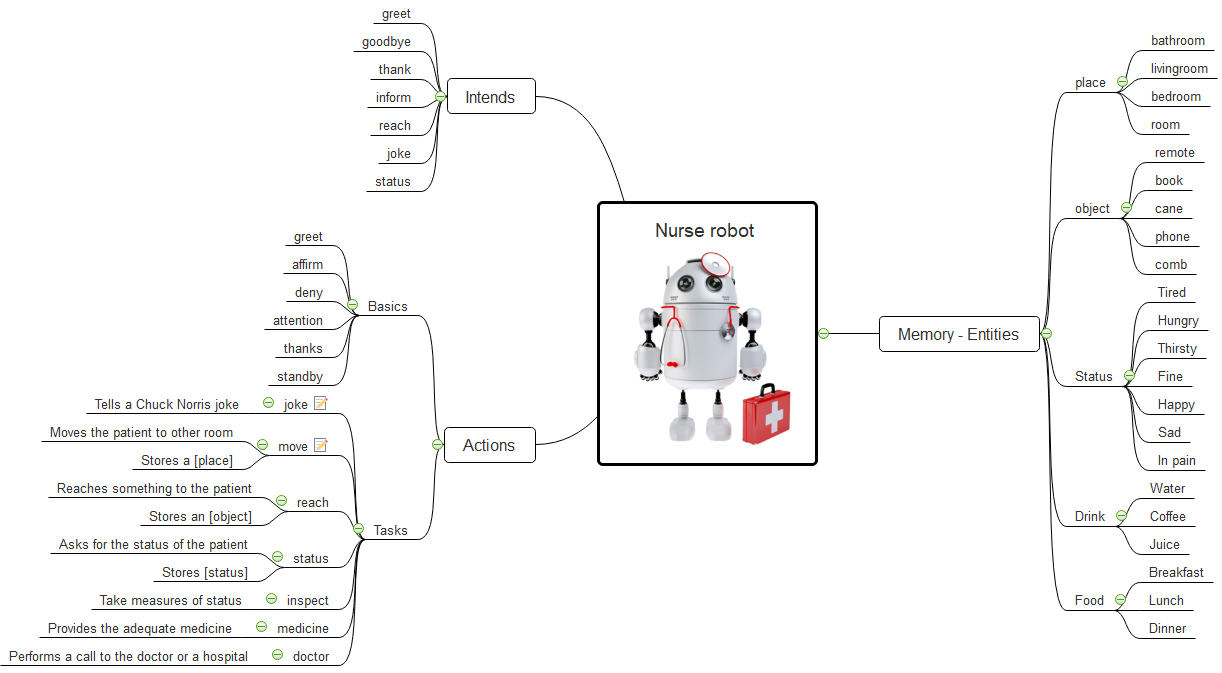
\includegraphics{images/NurseRobotMindmap.png}
\caption{title}
\end{figure}

    \begin{Verbatim}[commandchars=\\\{\}]
{\color{incolor}In [{\color{incolor}2}]:} \PY{c+c1}{\PYZsh{}imports for project}
        
        \PY{k+kn}{from} \PY{n+nn}{\PYZus{}\PYZus{}future\PYZus{}\PYZus{}} \PY{k}{import} \PY{n}{absolute\PYZus{}import}
        \PY{k+kn}{from} \PY{n+nn}{\PYZus{}\PYZus{}future\PYZus{}\PYZus{}} \PY{k}{import} \PY{n}{division}
        \PY{k+kn}{from} \PY{n+nn}{\PYZus{}\PYZus{}future\PYZus{}\PYZus{}} \PY{k}{import} \PY{n}{print\PYZus{}function}
        \PY{k+kn}{from} \PY{n+nn}{\PYZus{}\PYZus{}future\PYZus{}\PYZus{}} \PY{k}{import} \PY{n}{unicode\PYZus{}literals}
        
        \PY{k+kn}{import} \PY{n+nn}{logging}
        \PY{k+kn}{import} \PY{n+nn}{rasa\PYZus{}core}
        \PY{k+kn}{from} \PY{n+nn}{rasa\PYZus{}core}\PY{n+nn}{.}\PY{n+nn}{agent} \PY{k}{import} \PY{n}{Agent}
        \PY{k+kn}{from} \PY{n+nn}{rasa\PYZus{}core}\PY{n+nn}{.}\PY{n+nn}{policies}\PY{n+nn}{.}\PY{n+nn}{keras\PYZus{}policy} \PY{k}{import} \PY{n}{KerasPolicy}
        \PY{k+kn}{from} \PY{n+nn}{rasa\PYZus{}core}\PY{n+nn}{.}\PY{n+nn}{policies}\PY{n+nn}{.}\PY{n+nn}{memoization} \PY{k}{import} \PY{n}{MemoizationPolicy}
        \PY{k+kn}{from} \PY{n+nn}{rasa\PYZus{}core}\PY{n+nn}{.}\PY{n+nn}{interpreter} \PY{k}{import} \PY{n}{RasaNLUInterpreter}
        \PY{k+kn}{from} \PY{n+nn}{rasa\PYZus{}nlu}\PY{n+nn}{.}\PY{n+nn}{model} \PY{k}{import} \PY{n}{Metadata}\PY{p}{,} \PY{n}{Interpreter}
        \PY{k+kn}{from} \PY{n+nn}{rasa\PYZus{}core}\PY{n+nn}{.}\PY{n+nn}{utils} \PY{k}{import} \PY{n}{EndpointConfig}
        \PY{k+kn}{from} \PY{n+nn}{rasa\PYZus{}core}\PY{n+nn}{.}\PY{n+nn}{run} \PY{k}{import} \PY{n}{serve\PYZus{}application}
        \PY{k+kn}{from} \PY{n+nn}{rasa\PYZus{}nlu}\PY{n+nn}{.}\PY{n+nn}{model} \PY{k}{import} \PY{n}{Trainer}
        \PY{k+kn}{from} \PY{n+nn}{rasa\PYZus{}nlu}\PY{n+nn}{.}\PY{n+nn}{training\PYZus{}data} \PY{k}{import} \PY{n}{load\PYZus{}data}
        \PY{k+kn}{from} \PY{n+nn}{rasa\PYZus{}core} \PY{k}{import} \PY{n}{config}
        \PY{k+kn}{from} \PY{n+nn}{IPython}\PY{n+nn}{.}\PY{n+nn}{display} \PY{k}{import} \PY{n}{IFrame}
        \PY{k+kn}{import} \PY{n+nn}{pandas} \PY{k}{as} \PY{n+nn}{pd}
        \PY{k+kn}{import} \PY{n+nn}{ruamel}
        \PY{k+kn}{import} \PY{n+nn}{urllib}\PY{n+nn}{.}\PY{n+nn}{request}
        \PY{k+kn}{from} \PY{n+nn}{urllib}\PY{n+nn}{.}\PY{n+nn}{request} \PY{k}{import} \PY{n}{urlopen}
        \PY{k+kn}{from} \PY{n+nn}{playsound} \PY{k}{import} \PY{n}{playsound}
        \PY{k+kn}{import} \PY{n+nn}{uuid}
        \PY{k+kn}{import} \PY{n+nn}{speech\PYZus{}recognition} \PY{k}{as} \PY{n+nn}{sr}
        
        \PY{k+kn}{import} \PY{n+nn}{os}
        
        \PY{k+kn}{import} \PY{n+nn}{spacy}
        
        \PY{k+kn}{import} \PY{n+nn}{warnings}
        \PY{n}{warnings}\PY{o}{.}\PY{n}{simplefilter}\PY{p}{(}\PY{l+s+s1}{\PYZsq{}}\PY{l+s+s1}{ignore}\PY{l+s+s1}{\PYZsq{}}\PY{p}{,} \PY{n}{ruamel}\PY{o}{.}\PY{n}{yaml}\PY{o}{.}\PY{n}{error}\PY{o}{.}\PY{n}{UnsafeLoaderWarning}\PY{p}{)}
        \PY{n}{warnings}\PY{o}{.}\PY{n}{filterwarnings}\PY{p}{(}\PY{l+s+s2}{\PYZdq{}}\PY{l+s+s2}{ignore}\PY{l+s+s2}{\PYZdq{}}\PY{p}{,}\PY{n}{category}\PY{o}{=}\PY{n+ne}{DeprecationWarning}\PY{p}{)}
        \PY{n}{os}\PY{o}{.}\PY{n}{environ}\PY{p}{[}\PY{l+s+s1}{\PYZsq{}}\PY{l+s+s1}{TF\PYZus{}CPP\PYZus{}MIN\PYZus{}LOG\PYZus{}LEVEL}\PY{l+s+s1}{\PYZsq{}}\PY{p}{]} \PY{o}{=} \PY{l+s+s1}{\PYZsq{}}\PY{l+s+s1}{2}\PY{l+s+s1}{\PYZsq{}} \PY{c+c1}{\PYZsh{}To ignore Tensorflow AVX AVX2 bonary warning}
\end{Verbatim}


    Some of the data used in this project is not shown in this notebook, but
in external files. The content of each relevant file is described
hereunder.

\begin{itemize}
\tightlist
\item
  nurse\_domain.yml: Defines the actions that can be taken by the agent,
  the intents that are expected, the entities to be saved if received,
  and some answers to the basic user utterances.
\item
  stories.md: Contains the examples of dialogs and the specification of
  the entities that could be found on the phrases.
\item
  config\_spacy.json: Saves the pipeline to be used by the NLP library,
  in this case sklearn with spaCy
\end{itemize}

    \begin{Verbatim}[commandchars=\\\{\}]
{\color{incolor}In [{\color{incolor}3}]:} \PY{c+c1}{\PYZsh{} Declare paths}
        \PY{n}{domain\PYZus{}file} \PY{o}{=} \PY{l+s+s1}{\PYZsq{}}\PY{l+s+s1}{./nurse\PYZus{}domain.yml}\PY{l+s+s1}{\PYZsq{}}
        \PY{n}{model\PYZus{}path} \PY{o}{=} \PY{l+s+s1}{\PYZsq{}}\PY{l+s+s1}{./models/dialogue}\PY{l+s+s1}{\PYZsq{}}
        \PY{n}{interpreter\PYZus{}path} \PY{o}{=}\PY{l+s+s1}{\PYZsq{}}\PY{l+s+s1}{./models/nursebot/interpreter}\PY{l+s+s1}{\PYZsq{}}
        \PY{n}{training\PYZus{}data\PYZus{}file} \PY{o}{=} \PY{l+s+s1}{\PYZsq{}}\PY{l+s+s1}{./data/stories.md}\PY{l+s+s1}{\PYZsq{}}
        \PY{n}{conf\PYZus{}file} \PY{o}{=} \PY{l+s+s1}{\PYZsq{}}\PY{l+s+s1}{./config\PYZus{}spacy.json}\PY{l+s+s1}{\PYZsq{}}
\end{Verbatim}


    \begin{Verbatim}[commandchars=\\\{\}]
{\color{incolor}In [{\color{incolor}4}]:} \PY{c+c1}{\PYZsh{} Build the interpreter of the elements of dialog for the agent}
        \PY{o}{!}python \PYZhy{}m rasa\PYZus{}nlu.train \PYZhy{}c config\PYZus{}spacy.json \PYZhy{}\PYZhy{}data data/data.md \PYZhy{}o models \PYZhy{}\PYZhy{}fixed\PYZus{}model\PYZus{}name interpreter \PYZhy{}\PYZhy{}project nursebot \PYZhy{}\PYZhy{}verbose
\end{Verbatim}


    \begin{Verbatim}[commandchars=\\\{\}]
Fitting 2 folds for each of 6 candidates, totalling 12 fits

    \end{Verbatim}

    \begin{Verbatim}[commandchars=\\\{\}]
2019-01-22 18:06:02 INFO     rasa\_nlu.utils.spacy\_utils  - Trying to load spacy model with name 'en'
2019-01-22 18:06:06 INFO     rasa\_nlu.components  - Added 'nlp\_spacy' to component cache. Key 'nlp\_spacy-en'.
2019-01-22 18:06:06 INFO     rasa\_nlu.training\_data.loading  - Training data format of data/data.md is md
2019-01-22 18:06:06 INFO     rasa\_nlu.training\_data.training\_data  - Training data stats: 
	- intent examples: 103 (9 distinct intents)
	- Found intents: 'affirm', 'thanks', 'attention', 'deny', 'joke', 'greet', 'move', 'reach', 'goodbye'
	- entity examples: 29 (2 distinct entities)
	- found entities: 'object', 'place'

2019-01-22 18:06:06 INFO     rasa\_nlu.model  - Starting to train component nlp\_spacy
2019-01-22 18:06:07 INFO     rasa\_nlu.model  - Finished training component.
2019-01-22 18:06:07 INFO     rasa\_nlu.model  - Starting to train component tokenizer\_spacy
2019-01-22 18:06:07 INFO     rasa\_nlu.model  - Finished training component.
2019-01-22 18:06:07 INFO     rasa\_nlu.model  - Starting to train component intent\_featurizer\_spacy
2019-01-22 18:06:07 INFO     rasa\_nlu.model  - Finished training component.
2019-01-22 18:06:07 INFO     rasa\_nlu.model  - Starting to train component intent\_entity\_featurizer\_regex
2019-01-22 18:06:07 INFO     rasa\_nlu.model  - Finished training component.
2019-01-22 18:06:07 INFO     rasa\_nlu.model  - Starting to train component ner\_crf
2019-01-22 18:06:07 INFO     rasa\_nlu.model  - Finished training component.
2019-01-22 18:06:07 INFO     rasa\_nlu.model  - Starting to train component ner\_synonyms
2019-01-22 18:06:07 INFO     rasa\_nlu.model  - Finished training component.
2019-01-22 18:06:07 INFO     rasa\_nlu.model  - Starting to train component intent\_classifier\_sklearn
[Parallel(n\_jobs=1)]: Done  12 out of  12 | elapsed:    0.2s finished
2019-01-22 18:06:08 INFO     rasa\_nlu.model  - Finished training component.
2019-01-22 18:06:08 INFO     rasa\_nlu.model  - Successfully saved model into 'D:\textbackslash{}GoogleDrive\textbackslash{}MasterSapienza\textbackslash{}Semestre1\textbackslash{}AI\textbackslash{}Sec 2A\textbackslash{}Human Robot Interaction\textbackslash{}HRI-Project\textbackslash{}NurseRobotV1\textbackslash{}models\textbackslash{}nursebot\textbackslash{}interpreter'
2019-01-22 18:06:08 INFO     \_\_main\_\_  - Finished training

    \end{Verbatim}

    \begin{Verbatim}[commandchars=\\\{\}]
{\color{incolor}In [{\color{incolor}5}]:} \PY{n}{action\PYZus{}endpoint} \PY{o}{=} \PY{n}{EndpointConfig}\PY{p}{(}\PY{n}{url}\PY{o}{=}\PY{l+s+s2}{\PYZdq{}}\PY{l+s+s2}{http://localhost:5055/webhook}\PY{l+s+s2}{\PYZdq{}}\PY{p}{)}
        \PY{n}{interpreter} \PY{o}{=} \PY{n}{RasaNLUInterpreter}\PY{p}{(}\PY{n}{interpreter\PYZus{}path}\PY{p}{)}
        
        \PY{n}{agent} \PY{o}{=} \PY{n}{Agent}\PY{p}{(}\PY{n}{domain\PYZus{}file}\PY{p}{,} 
                      \PY{n}{policies} \PY{o}{=} \PY{p}{[}\PY{n}{MemoizationPolicy}\PY{p}{(}\PY{p}{)}\PY{p}{,} \PY{n}{KerasPolicy}\PY{p}{(}\PY{n}{max\PYZus{}history}\PY{o}{=}\PY{l+m+mi}{3}\PY{p}{,} \PY{n}{epochs}\PY{o}{=}\PY{l+m+mi}{200}\PY{p}{,} \PY{n}{batch\PYZus{}size}\PY{o}{=}\PY{l+m+mi}{50}\PY{p}{)}\PY{p}{]}\PY{p}{,}
                      \PY{n}{interpreter}\PY{o}{=}\PY{n}{interpreter}\PY{p}{,}
                      \PY{n}{action\PYZus{}endpoint}\PY{o}{=}\PY{n}{action\PYZus{}endpoint}\PY{p}{)}
        \PY{n}{data} \PY{o}{=} \PY{n}{agent}\PY{o}{.}\PY{n}{load\PYZus{}data}\PY{p}{(}\PY{n}{training\PYZus{}data\PYZus{}file}\PY{p}{)}
        \PY{n}{agent}\PY{o}{.}\PY{n}{train}\PY{p}{(}\PY{n}{data}\PY{p}{)}
\end{Verbatim}


    \begin{Verbatim}[commandchars=\\\{\}]
C:\textbackslash{}Users\textbackslash{}AndresArciniegas\textbackslash{}AppData\textbackslash{}Roaming\textbackslash{}Python\textbackslash{}Python36\textbackslash{}site-packages\textbackslash{}rasa\_nlu\textbackslash{}extractors\textbackslash{}entity\_synonyms.py:85: UserWarning: Failed to load synonyms file from './models/nursebot/interpreter\textbackslash{}entity\_synonyms.json'
  "".format(entity\_synonyms\_file))
Processed Story Blocks: 100\%|███████████████████████████████████████████| 21/21 [00:00<00:00, 447.99it/s, \# trackers=1]
Processed Story Blocks: 100\%|██████████████████████████████████████████| 21/21 [00:00<00:00, 189.72it/s, \# trackers=19]
Processed Story Blocks: 100\%|██████████████████████████████████████████| 21/21 [00:00<00:00, 202.46it/s, \# trackers=19]
Processed Story Blocks: 100\%|██████████████████████████████████████████| 21/21 [00:00<00:00, 129.18it/s, \# trackers=18]
Processed actions: 1440it [00:02, 554.99it/s, \# examples=1440]

    \end{Verbatim}

    \begin{Verbatim}[commandchars=\\\{\}]
\_\_\_\_\_\_\_\_\_\_\_\_\_\_\_\_\_\_\_\_\_\_\_\_\_\_\_\_\_\_\_\_\_\_\_\_\_\_\_\_\_\_\_\_\_\_\_\_\_\_\_\_\_\_\_\_\_\_\_\_\_\_\_\_\_
Layer (type)                 Output Shape              Param \#   
=================================================================
masking (Masking)            (None, 3, 27)             0         
\_\_\_\_\_\_\_\_\_\_\_\_\_\_\_\_\_\_\_\_\_\_\_\_\_\_\_\_\_\_\_\_\_\_\_\_\_\_\_\_\_\_\_\_\_\_\_\_\_\_\_\_\_\_\_\_\_\_\_\_\_\_\_\_\_
lstm (LSTM)                  (None, 32)                7680      
\_\_\_\_\_\_\_\_\_\_\_\_\_\_\_\_\_\_\_\_\_\_\_\_\_\_\_\_\_\_\_\_\_\_\_\_\_\_\_\_\_\_\_\_\_\_\_\_\_\_\_\_\_\_\_\_\_\_\_\_\_\_\_\_\_
dense (Dense)                (None, 13)                429       
\_\_\_\_\_\_\_\_\_\_\_\_\_\_\_\_\_\_\_\_\_\_\_\_\_\_\_\_\_\_\_\_\_\_\_\_\_\_\_\_\_\_\_\_\_\_\_\_\_\_\_\_\_\_\_\_\_\_\_\_\_\_\_\_\_
activation (Activation)      (None, 13)                0         
=================================================================
Total params: 8,109
Trainable params: 8,109
Non-trainable params: 0
\_\_\_\_\_\_\_\_\_\_\_\_\_\_\_\_\_\_\_\_\_\_\_\_\_\_\_\_\_\_\_\_\_\_\_\_\_\_\_\_\_\_\_\_\_\_\_\_\_\_\_\_\_\_\_\_\_\_\_\_\_\_\_\_\_
Epoch 1/200
625/625 [==============================] - ETA: 17s - loss: 2.5831 - acc: 0.10 - ETA: 4s - loss: 2.5514 - acc: 0.1400 - 2s 3ms/step - loss: 2.5109 - acc: 0.2064
Epoch 2/200
625/625 [==============================] - ETA: 0s - loss: 2.4660 - acc: 0.280 - 0s 85us/step - loss: 2.3956 - acc: 0.3984
Epoch 3/200
625/625 [==============================] - ETA: 0s - loss: 2.3858 - acc: 0.340 - 0s 78us/step - loss: 2.2773 - acc: 0.4400
Epoch 4/200
625/625 [==============================] - ETA: 0s - loss: 2.1847 - acc: 0.480 - 0s 77us/step - loss: 2.1348 - acc: 0.4400
Epoch 5/200
625/625 [==============================] - ETA: 0s - loss: 1.9677 - acc: 0.560 - 0s 70us/step - loss: 2.0147 - acc: 0.4400
Epoch 6/200
625/625 [==============================] - ETA: 0s - loss: 2.0240 - acc: 0.420 - 0s 67us/step - loss: 1.9285 - acc: 0.4400
Epoch 7/200
625/625 [==============================] - ETA: 0s - loss: 1.9544 - acc: 0.420 - 0s 77us/step - loss: 1.8622 - acc: 0.4400
Epoch 8/200
625/625 [==============================] - ETA: 0s - loss: 1.5498 - acc: 0.560 - 0s 72us/step - loss: 1.8231 - acc: 0.4432
Epoch 9/200
625/625 [==============================] - ETA: 0s - loss: 1.8344 - acc: 0.440 - 0s 77us/step - loss: 1.7736 - acc: 0.4400
Epoch 10/200
625/625 [==============================] - ETA: 0s - loss: 1.6733 - acc: 0.540 - 0s 81us/step - loss: 1.7377 - acc: 0.4416
Epoch 11/200
625/625 [==============================] - ETA: 0s - loss: 1.8204 - acc: 0.360 - 0s 73us/step - loss: 1.6934 - acc: 0.4528
Epoch 12/200
625/625 [==============================] - ETA: 0s - loss: 1.3880 - acc: 0.560 - 0s 73us/step - loss: 1.6424 - acc: 0.4624
Epoch 13/200
625/625 [==============================] - ETA: 0s - loss: 1.5137 - acc: 0.540 - 0s 72us/step - loss: 1.6018 - acc: 0.4752
Epoch 14/200
625/625 [==============================] - ETA: 0s - loss: 1.4989 - acc: 0.520 - 0s 69us/step - loss: 1.5572 - acc: 0.4768
Epoch 15/200
625/625 [==============================] - ETA: 0s - loss: 1.6034 - acc: 0.500 - 0s 72us/step - loss: 1.5166 - acc: 0.4928
Epoch 16/200
625/625 [==============================] - ETA: 0s - loss: 1.7795 - acc: 0.400 - 0s 73us/step - loss: 1.4774 - acc: 0.4976
Epoch 17/200
625/625 [==============================] - ETA: 0s - loss: 1.4416 - acc: 0.500 - 0s 73us/step - loss: 1.4445 - acc: 0.5008
Epoch 18/200
625/625 [==============================] - ETA: 0s - loss: 1.3623 - acc: 0.520 - 0s 80us/step - loss: 1.4080 - acc: 0.4992
Epoch 19/200
625/625 [==============================] - ETA: 0s - loss: 1.4128 - acc: 0.480 - 0s 81us/step - loss: 1.3420 - acc: 0.5168
Epoch 20/200
625/625 [==============================] - ETA: 0s - loss: 1.6861 - acc: 0.400 - 0s 72us/step - loss: 1.2993 - acc: 0.5392
Epoch 21/200
625/625 [==============================] - ETA: 0s - loss: 1.4624 - acc: 0.380 - 0s 73us/step - loss: 1.2516 - acc: 0.5312
Epoch 22/200
625/625 [==============================] - ETA: 0s - loss: 1.0579 - acc: 0.660 - 0s 77us/step - loss: 1.1985 - acc: 0.5728
Epoch 23/200
625/625 [==============================] - ETA: 0s - loss: 1.2213 - acc: 0.540 - 0s 73us/step - loss: 1.1093 - acc: 0.6272
Epoch 24/200
625/625 [==============================] - ETA: 0s - loss: 1.1182 - acc: 0.680 - 0s 73us/step - loss: 1.0582 - acc: 0.6560
Epoch 25/200
625/625 [==============================] - ETA: 0s - loss: 1.0831 - acc: 0.700 - 0s 70us/step - loss: 1.0197 - acc: 0.6960
Epoch 26/200
625/625 [==============================] - ETA: 0s - loss: 1.1231 - acc: 0.560 - 0s 65us/step - loss: 0.9374 - acc: 0.7232
Epoch 27/200
625/625 [==============================] - ETA: 0s - loss: 0.8541 - acc: 0.740 - 0s 70us/step - loss: 0.8897 - acc: 0.7536
Epoch 28/200
625/625 [==============================] - ETA: 0s - loss: 0.9078 - acc: 0.780 - 0s 78us/step - loss: 0.8500 - acc: 0.7856
Epoch 29/200
625/625 [==============================] - ETA: 0s - loss: 0.8792 - acc: 0.780 - 0s 73us/step - loss: 0.7847 - acc: 0.8112
Epoch 30/200
625/625 [==============================] - ETA: 0s - loss: 0.6919 - acc: 0.840 - 0s 72us/step - loss: 0.7352 - acc: 0.8304
Epoch 31/200
625/625 [==============================] - ETA: 0s - loss: 0.7741 - acc: 0.820 - 0s 73us/step - loss: 0.6816 - acc: 0.8416
Epoch 32/200
625/625 [==============================] - ETA: 0s - loss: 0.7437 - acc: 0.820 - 0s 69us/step - loss: 0.6786 - acc: 0.8448
Epoch 33/200
625/625 [==============================] - ETA: 0s - loss: 0.6364 - acc: 0.880 - 0s 75us/step - loss: 0.6412 - acc: 0.8720
Epoch 34/200
625/625 [==============================] - ETA: 0s - loss: 0.5080 - acc: 0.920 - 0s 82us/step - loss: 0.6014 - acc: 0.8832
Epoch 35/200
625/625 [==============================] - ETA: 0s - loss: 0.5941 - acc: 0.920 - 0s 73us/step - loss: 0.5676 - acc: 0.9008
Epoch 36/200
625/625 [==============================] - ETA: 0s - loss: 0.6561 - acc: 0.900 - 0s 77us/step - loss: 0.5331 - acc: 0.9040
Epoch 37/200
625/625 [==============================] - ETA: 0s - loss: 0.4257 - acc: 0.980 - 0s 69us/step - loss: 0.5230 - acc: 0.9104
Epoch 38/200
625/625 [==============================] - ETA: 0s - loss: 0.5329 - acc: 0.940 - 0s 82us/step - loss: 0.4983 - acc: 0.9152
Epoch 39/200
625/625 [==============================] - ETA: 0s - loss: 0.5396 - acc: 0.900 - 0s 83us/step - loss: 0.4669 - acc: 0.9216
Epoch 40/200
625/625 [==============================] - ETA: 0s - loss: 0.5822 - acc: 0.880 - 0s 89us/step - loss: 0.4507 - acc: 0.9104
Epoch 41/200
625/625 [==============================] - ETA: 0s - loss: 0.5151 - acc: 0.900 - 0s 77us/step - loss: 0.4277 - acc: 0.9184
Epoch 42/200
625/625 [==============================] - ETA: 0s - loss: 0.3711 - acc: 0.920 - 0s 78us/step - loss: 0.4159 - acc: 0.9264
Epoch 43/200
625/625 [==============================] - ETA: 0s - loss: 0.4114 - acc: 0.900 - 0s 89us/step - loss: 0.3985 - acc: 0.9184
Epoch 44/200
625/625 [==============================] - ETA: 0s - loss: 0.3647 - acc: 0.940 - 0s 75us/step - loss: 0.3603 - acc: 0.9280
Epoch 45/200
625/625 [==============================] - ETA: 0s - loss: 0.2809 - acc: 0.960 - 0s 83us/step - loss: 0.3453 - acc: 0.9440
Epoch 46/200
625/625 [==============================] - ETA: 0s - loss: 0.3300 - acc: 0.920 - 0s 77us/step - loss: 0.3851 - acc: 0.9184
Epoch 47/200
625/625 [==============================] - ETA: 0s - loss: 0.3729 - acc: 0.920 - 0s 80us/step - loss: 0.3531 - acc: 0.9360
Epoch 48/200
625/625 [==============================] - ETA: 0s - loss: 0.3784 - acc: 0.940 - 0s 77us/step - loss: 0.3457 - acc: 0.9264
Epoch 49/200
625/625 [==============================] - ETA: 0s - loss: 0.3950 - acc: 0.880 - 0s 78us/step - loss: 0.3288 - acc: 0.9360
Epoch 50/200
625/625 [==============================] - ETA: 0s - loss: 0.2690 - acc: 0.980 - 0s 73us/step - loss: 0.2891 - acc: 0.9424
Epoch 51/200
625/625 [==============================] - ETA: 0s - loss: 0.4868 - acc: 0.900 - 0s 67us/step - loss: 0.3142 - acc: 0.9232
Epoch 52/200
625/625 [==============================] - ETA: 0s - loss: 0.1457 - acc: 1.000 - 0s 70us/step - loss: 0.2810 - acc: 0.9408
Epoch 53/200
625/625 [==============================] - ETA: 0s - loss: 0.2640 - acc: 0.960 - 0s 67us/step - loss: 0.3055 - acc: 0.9296
Epoch 54/200
625/625 [==============================] - ETA: 0s - loss: 0.2443 - acc: 0.960 - 0s 75us/step - loss: 0.2750 - acc: 0.9376
Epoch 55/200
625/625 [==============================] - ETA: 0s - loss: 0.2243 - acc: 0.980 - 0s 77us/step - loss: 0.2466 - acc: 0.9440
Epoch 56/200
625/625 [==============================] - ETA: 0s - loss: 0.2657 - acc: 0.960 - 0s 73us/step - loss: 0.2323 - acc: 0.9504
Epoch 57/200
625/625 [==============================] - ETA: 0s - loss: 0.2356 - acc: 0.940 - 0s 75us/step - loss: 0.2506 - acc: 0.9408
Epoch 58/200
625/625 [==============================] - ETA: 0s - loss: 0.2846 - acc: 0.920 - 0s 72us/step - loss: 0.2509 - acc: 0.9440
Epoch 59/200
625/625 [==============================] - ETA: 0s - loss: 0.2669 - acc: 0.940 - 0s 69us/step - loss: 0.2328 - acc: 0.9472
Epoch 60/200
625/625 [==============================] - ETA: 0s - loss: 0.2272 - acc: 0.940 - 0s 67us/step - loss: 0.2089 - acc: 0.9488
Epoch 61/200
625/625 [==============================] - ETA: 0s - loss: 0.2958 - acc: 0.880 - 0s 72us/step - loss: 0.2215 - acc: 0.9472
Epoch 62/200
625/625 [==============================] - ETA: 0s - loss: 0.2659 - acc: 0.900 - 0s 73us/step - loss: 0.2259 - acc: 0.9456
Epoch 63/200
625/625 [==============================] - ETA: 0s - loss: 0.3163 - acc: 0.940 - 0s 78us/step - loss: 0.2067 - acc: 0.9456
Epoch 64/200
625/625 [==============================] - ETA: 0s - loss: 0.3094 - acc: 0.920 - 0s 72us/step - loss: 0.2144 - acc: 0.9504
Epoch 65/200
625/625 [==============================] - ETA: 0s - loss: 0.1743 - acc: 0.940 - 0s 64us/step - loss: 0.2106 - acc: 0.9424
Epoch 66/200
625/625 [==============================] - ETA: 0s - loss: 0.2282 - acc: 0.920 - 0s 71us/step - loss: 0.2052 - acc: 0.9504
Epoch 67/200
625/625 [==============================] - ETA: 0s - loss: 0.1440 - acc: 0.980 - 0s 86us/step - loss: 0.1891 - acc: 0.9552
Epoch 68/200
625/625 [==============================] - ETA: 0s - loss: 0.1832 - acc: 0.960 - 0s 70us/step - loss: 0.2128 - acc: 0.9424
Epoch 69/200
625/625 [==============================] - ETA: 0s - loss: 0.2784 - acc: 0.900 - 0s 70us/step - loss: 0.1792 - acc: 0.9568
Epoch 70/200
625/625 [==============================] - ETA: 0s - loss: 0.1866 - acc: 0.980 - 0s 69us/step - loss: 0.1876 - acc: 0.9520
Epoch 71/200
625/625 [==============================] - ETA: 0s - loss: 0.1358 - acc: 0.960 - 0s 64us/step - loss: 0.1730 - acc: 0.9600
Epoch 72/200
625/625 [==============================] - ETA: 0s - loss: 0.1653 - acc: 0.920 - 0s 70us/step - loss: 0.1699 - acc: 0.9584
Epoch 73/200
625/625 [==============================] - ETA: 0s - loss: 0.2046 - acc: 0.940 - 0s 70us/step - loss: 0.1568 - acc: 0.9584
Epoch 74/200
625/625 [==============================] - ETA: 0s - loss: 0.1315 - acc: 0.980 - 0s 70us/step - loss: 0.1769 - acc: 0.9584
Epoch 75/200
625/625 [==============================] - ETA: 0s - loss: 0.1309 - acc: 1.000 - 0s 70us/step - loss: 0.1468 - acc: 0.9664
Epoch 76/200
625/625 [==============================] - ETA: 0s - loss: 0.1280 - acc: 0.960 - 0s 70us/step - loss: 0.1709 - acc: 0.9536
Epoch 77/200
625/625 [==============================] - ETA: 0s - loss: 0.1601 - acc: 0.980 - 0s 70us/step - loss: 0.1328 - acc: 0.9744
Epoch 78/200
625/625 [==============================] - ETA: 0s - loss: 0.1364 - acc: 0.960 - 0s 72us/step - loss: 0.1223 - acc: 0.9760
Epoch 79/200
625/625 [==============================] - ETA: 0s - loss: 0.1911 - acc: 1.000 - 0s 78us/step - loss: 0.1526 - acc: 0.9648
Epoch 80/200
625/625 [==============================] - ETA: 0s - loss: 0.2145 - acc: 0.940 - 0s 70us/step - loss: 0.1638 - acc: 0.9584
Epoch 81/200
625/625 [==============================] - ETA: 0s - loss: 0.1145 - acc: 0.960 - 0s 69us/step - loss: 0.1645 - acc: 0.9568
Epoch 82/200
625/625 [==============================] - ETA: 0s - loss: 0.0833 - acc: 0.980 - 0s 83us/step - loss: 0.1617 - acc: 0.9584
Epoch 83/200
625/625 [==============================] - ETA: 0s - loss: 0.1495 - acc: 0.940 - ETA: 0s - loss: 0.1408 - acc: 0.967 - 0s 112us/step - loss: 0.1468 - acc: 0.9632
Epoch 84/200
625/625 [==============================] - ETA: 0s - loss: 0.1035 - acc: 0.960 - 0s 97us/step - loss: 0.1570 - acc: 0.9632
Epoch 85/200
625/625 [==============================] - ETA: 0s - loss: 0.0928 - acc: 0.980 - ETA: 0s - loss: 0.1540 - acc: 0.956 - 0s 101us/step - loss: 0.1595 - acc: 0.9536
Epoch 86/200
625/625 [==============================] - ETA: 0s - loss: 0.3122 - acc: 0.920 - 0s 94us/step - loss: 0.1549 - acc: 0.9664
Epoch 87/200
625/625 [==============================] - ETA: 0s - loss: 0.1271 - acc: 0.980 - 0s 77us/step - loss: 0.1397 - acc: 0.9648
Epoch 88/200
625/625 [==============================] - ETA: 0s - loss: 0.1520 - acc: 0.960 - 0s 80us/step - loss: 0.1602 - acc: 0.9616
Epoch 89/200
625/625 [==============================] - ETA: 0s - loss: 0.0630 - acc: 1.000 - 0s 80us/step - loss: 0.1277 - acc: 0.9744
Epoch 90/200
625/625 [==============================] - ETA: 0s - loss: 0.0571 - acc: 0.980 - 0s 72us/step - loss: 0.1275 - acc: 0.9648
Epoch 91/200
625/625 [==============================] - ETA: 0s - loss: 0.1111 - acc: 0.980 - 0s 78us/step - loss: 0.1278 - acc: 0.9728
Epoch 92/200
625/625 [==============================] - ETA: 0s - loss: 0.1154 - acc: 0.980 - 0s 89us/step - loss: 0.1215 - acc: 0.9728
Epoch 93/200
625/625 [==============================] - ETA: 0s - loss: 0.0752 - acc: 0.980 - 0s 69us/step - loss: 0.1236 - acc: 0.9664
Epoch 94/200
625/625 [==============================] - ETA: 0s - loss: 0.2092 - acc: 0.940 - 0s 67us/step - loss: 0.1201 - acc: 0.9728
Epoch 95/200
625/625 [==============================] - ETA: 0s - loss: 0.1330 - acc: 0.980 - 0s 70us/step - loss: 0.1160 - acc: 0.9696
Epoch 96/200
625/625 [==============================] - ETA: 0s - loss: 0.0857 - acc: 0.980 - 0s 77us/step - loss: 0.0992 - acc: 0.9776
Epoch 97/200
625/625 [==============================] - ETA: 0s - loss: 0.0559 - acc: 0.980 - 0s 75us/step - loss: 0.1234 - acc: 0.9792
Epoch 98/200
625/625 [==============================] - ETA: 0s - loss: 0.1389 - acc: 0.980 - 0s 70us/step - loss: 0.1407 - acc: 0.9680
Epoch 99/200
625/625 [==============================] - ETA: 0s - loss: 0.0683 - acc: 0.980 - 0s 72us/step - loss: 0.1107 - acc: 0.9728
Epoch 100/200
625/625 [==============================] - ETA: 0s - loss: 0.1129 - acc: 0.980 - 0s 72us/step - loss: 0.1113 - acc: 0.9728
Epoch 101/200
625/625 [==============================] - ETA: 0s - loss: 0.0839 - acc: 0.980 - 0s 67us/step - loss: 0.1139 - acc: 0.9760
Epoch 102/200
625/625 [==============================] - ETA: 0s - loss: 0.0666 - acc: 0.980 - 0s 67us/step - loss: 0.1124 - acc: 0.9728
Epoch 103/200
625/625 [==============================] - ETA: 0s - loss: 0.1274 - acc: 0.960 - 0s 67us/step - loss: 0.1007 - acc: 0.9744
Epoch 104/200
625/625 [==============================] - ETA: 0s - loss: 0.0791 - acc: 0.980 - 0s 70us/step - loss: 0.1245 - acc: 0.9712
Epoch 105/200
625/625 [==============================] - ETA: 0s - loss: 0.0897 - acc: 0.980 - 0s 71us/step - loss: 0.1195 - acc: 0.9728
Epoch 106/200
625/625 [==============================] - ETA: 0s - loss: 0.2197 - acc: 0.960 - ETA: 0s - loss: 0.1078 - acc: 0.981 - 0s 116us/step - loss: 0.1078 - acc: 0.9824
Epoch 107/200
625/625 [==============================] - ETA: 0s - loss: 0.1533 - acc: 0.980 - 0s 94us/step - loss: 0.0842 - acc: 0.9792
Epoch 108/200
625/625 [==============================] - ETA: 0s - loss: 0.1143 - acc: 0.980 - 0s 72us/step - loss: 0.0926 - acc: 0.9792
Epoch 109/200
625/625 [==============================] - ETA: 0s - loss: 0.1987 - acc: 0.960 - 0s 73us/step - loss: 0.1364 - acc: 0.9648
Epoch 110/200
625/625 [==============================] - ETA: 0s - loss: 0.0742 - acc: 1.000 - 0s 80us/step - loss: 0.0994 - acc: 0.9840
Epoch 111/200
625/625 [==============================] - ETA: 0s - loss: 0.0963 - acc: 1.000 - 0s 80us/step - loss: 0.1100 - acc: 0.9808
Epoch 112/200
625/625 [==============================] - ETA: 0s - loss: 0.0193 - acc: 1.000 - 0s 77us/step - loss: 0.0920 - acc: 0.9808
Epoch 113/200
625/625 [==============================] - ETA: 0s - loss: 0.0282 - acc: 1.000 - 0s 70us/step - loss: 0.0893 - acc: 0.9840
Epoch 114/200
625/625 [==============================] - ETA: 0s - loss: 0.1487 - acc: 0.960 - 0s 70us/step - loss: 0.0888 - acc: 0.9808
Epoch 115/200
625/625 [==============================] - ETA: 0s - loss: 0.1371 - acc: 0.940 - 0s 70us/step - loss: 0.0987 - acc: 0.9760
Epoch 116/200
625/625 [==============================] - ETA: 0s - loss: 0.0492 - acc: 1.000 - 0s 84us/step - loss: 0.0867 - acc: 0.9824
Epoch 117/200
625/625 [==============================] - ETA: 0s - loss: 0.0544 - acc: 1.000 - 0s 88us/step - loss: 0.1191 - acc: 0.9776
Epoch 118/200
625/625 [==============================] - ETA: 0s - loss: 0.0264 - acc: 1.000 - 0s 84us/step - loss: 0.0967 - acc: 0.9728
Epoch 119/200
625/625 [==============================] - ETA: 0s - loss: 0.1771 - acc: 0.940 - 0s 70us/step - loss: 0.1008 - acc: 0.9728
Epoch 120/200
625/625 [==============================] - ETA: 0s - loss: 0.1456 - acc: 0.940 - 0s 72us/step - loss: 0.1088 - acc: 0.9760
Epoch 121/200
625/625 [==============================] - ETA: 0s - loss: 0.2573 - acc: 0.920 - 0s 85us/step - loss: 0.1041 - acc: 0.9776
Epoch 122/200
625/625 [==============================] - ETA: 0s - loss: 0.0975 - acc: 0.940 - 0s 89us/step - loss: 0.0784 - acc: 0.9824
Epoch 123/200
625/625 [==============================] - ETA: 0s - loss: 0.0696 - acc: 1.000 - ETA: 0s - loss: 0.0935 - acc: 0.982 - 0s 137us/step - loss: 0.1013 - acc: 0.9792
Epoch 124/200
625/625 [==============================] - ETA: 0s - loss: 0.0928 - acc: 1.000 - ETA: 0s - loss: 0.0932 - acc: 0.980 - 0s 152us/step - loss: 0.0870 - acc: 0.9808
Epoch 125/200
625/625 [==============================] - ETA: 0s - loss: 0.1572 - acc: 0.940 - 0s 91us/step - loss: 0.0983 - acc: 0.9808
Epoch 126/200
625/625 [==============================] - ETA: 0s - loss: 0.0681 - acc: 0.980 - ETA: 0s - loss: 0.0721 - acc: 0.985 - 0s 105us/step - loss: 0.0763 - acc: 0.9856
Epoch 127/200
625/625 [==============================] - ETA: 0s - loss: 0.0563 - acc: 0.980 - ETA: 0s - loss: 0.0872 - acc: 0.973 - 0s 110us/step - loss: 0.0849 - acc: 0.9744
Epoch 128/200
625/625 [==============================] - ETA: 0s - loss: 0.1574 - acc: 0.980 - 0s 89us/step - loss: 0.0740 - acc: 0.9856
Epoch 129/200
625/625 [==============================] - ETA: 0s - loss: 0.0115 - acc: 1.000 - 0s 91us/step - loss: 0.0618 - acc: 0.9904
Epoch 130/200
625/625 [==============================] - ETA: 0s - loss: 0.0492 - acc: 0.980 - ETA: 0s - loss: 0.0826 - acc: 0.980 - 0s 116us/step - loss: 0.0885 - acc: 0.9792
Epoch 131/200
625/625 [==============================] - ETA: 0s - loss: 0.1239 - acc: 0.980 - ETA: 0s - loss: 0.0904 - acc: 0.978 - 0s 134us/step - loss: 0.0825 - acc: 0.9792
Epoch 132/200
625/625 [==============================] - ETA: 0s - loss: 0.0222 - acc: 1.000 - 0s 85us/step - loss: 0.0673 - acc: 0.9888
Epoch 133/200
625/625 [==============================] - ETA: 0s - loss: 0.0550 - acc: 0.980 - 0s 85us/step - loss: 0.0776 - acc: 0.9840
Epoch 134/200
625/625 [==============================] - ETA: 0s - loss: 0.0339 - acc: 1.000 - ETA: 0s - loss: 0.0742 - acc: 0.980 - 0s 123us/step - loss: 0.0738 - acc: 0.9808
Epoch 135/200
625/625 [==============================] - ETA: 0s - loss: 0.0123 - acc: 1.000 - 0s 76us/step - loss: 0.0605 - acc: 0.9920
Epoch 136/200
625/625 [==============================] - ETA: 0s - loss: 0.1004 - acc: 1.000 - 0s 77us/step - loss: 0.0638 - acc: 0.9856
Epoch 137/200
625/625 [==============================] - ETA: 0s - loss: 0.0355 - acc: 0.980 - 0s 75us/step - loss: 0.0650 - acc: 0.9872
Epoch 138/200
625/625 [==============================] - ETA: 0s - loss: 0.0417 - acc: 1.000 - 0s 65us/step - loss: 0.0918 - acc: 0.9760
Epoch 139/200
625/625 [==============================] - ETA: 0s - loss: 0.0854 - acc: 1.000 - ETA: 0s - loss: 0.0806 - acc: 0.977 - 0s 169us/step - loss: 0.0866 - acc: 0.9792
Epoch 140/200
625/625 [==============================] - ETA: 0s - loss: 0.1120 - acc: 0.960 - 0s 94us/step - loss: 0.0964 - acc: 0.9776
Epoch 141/200
625/625 [==============================] - ETA: 0s - loss: 0.0810 - acc: 0.980 - 0s 69us/step - loss: 0.0837 - acc: 0.9840
Epoch 142/200
625/625 [==============================] - ETA: 0s - loss: 0.0303 - acc: 1.000 - 0s 80us/step - loss: 0.0735 - acc: 0.9856
Epoch 143/200
625/625 [==============================] - ETA: 0s - loss: 0.0430 - acc: 1.000 - ETA: 0s - loss: 0.0876 - acc: 0.978 - 0s 125us/step - loss: 0.0868 - acc: 0.9776
Epoch 144/200
625/625 [==============================] - ETA: 0s - loss: 0.0283 - acc: 1.000 - ETA: 0s - loss: 0.0695 - acc: 0.983 - 0s 109us/step - loss: 0.0671 - acc: 0.9840
Epoch 145/200
625/625 [==============================] - ETA: 0s - loss: 0.0526 - acc: 1.000 - 0s 86us/step - loss: 0.0531 - acc: 0.9952
Epoch 146/200
625/625 [==============================] - ETA: 0s - loss: 0.1512 - acc: 0.960 - ETA: 0s - loss: 0.0611 - acc: 0.987 - 0s 109us/step - loss: 0.0624 - acc: 0.9872
Epoch 147/200
625/625 [==============================] - ETA: 0s - loss: 0.0975 - acc: 0.980 - ETA: 0s - loss: 0.0589 - acc: 0.988 - 0s 104us/step - loss: 0.0593 - acc: 0.9888
Epoch 148/200
625/625 [==============================] - ETA: 0s - loss: 0.0806 - acc: 1.000 - 0s 88us/step - loss: 0.0502 - acc: 0.9920
Epoch 149/200
625/625 [==============================] - ETA: 0s - loss: 0.0688 - acc: 0.980 - 0s 88us/step - loss: 0.0713 - acc: 0.9824
Epoch 150/200
625/625 [==============================] - ETA: 0s - loss: 0.0258 - acc: 1.000 - 0s 77us/step - loss: 0.0569 - acc: 0.9888
Epoch 151/200
625/625 [==============================] - ETA: 0s - loss: 0.0602 - acc: 0.980 - 0s 85us/step - loss: 0.0608 - acc: 0.9872
Epoch 152/200
625/625 [==============================] - ETA: 0s - loss: 0.0642 - acc: 1.000 - 0s 86us/step - loss: 0.0823 - acc: 0.9776
Epoch 153/200
625/625 [==============================] - ETA: 0s - loss: 0.0083 - acc: 1.000 - 0s 93us/step - loss: 0.0579 - acc: 0.9824
Epoch 154/200
625/625 [==============================] - ETA: 0s - loss: 0.1337 - acc: 0.960 - 0s 93us/step - loss: 0.0560 - acc: 0.9920
Epoch 155/200
625/625 [==============================] - ETA: 0s - loss: 0.0312 - acc: 1.000 - 0s 85us/step - loss: 0.0743 - acc: 0.9824
Epoch 156/200
625/625 [==============================] - ETA: 0s - loss: 0.0569 - acc: 0.980 - 0s 93us/step - loss: 0.0653 - acc: 0.9856
Epoch 157/200
625/625 [==============================] - ETA: 0s - loss: 0.0462 - acc: 1.000 - ETA: 0s - loss: 0.0578 - acc: 0.988 - 0s 124us/step - loss: 0.0613 - acc: 0.9824
Epoch 158/200
625/625 [==============================] - ETA: 0s - loss: 0.0505 - acc: 1.000 - ETA: 0s - loss: 0.0616 - acc: 0.988 - 0s 122us/step - loss: 0.0610 - acc: 0.9872
Epoch 159/200
625/625 [==============================] - ETA: 0s - loss: 0.0342 - acc: 1.000 - 0s 86us/step - loss: 0.0503 - acc: 0.9904
Epoch 160/200
625/625 [==============================] - ETA: 0s - loss: 0.0749 - acc: 0.980 - 0s 99us/step - loss: 0.0651 - acc: 0.9856
Epoch 161/200
625/625 [==============================] - ETA: 0s - loss: 0.0679 - acc: 0.960 - 0s 86us/step - loss: 0.0592 - acc: 0.9888
Epoch 162/200
625/625 [==============================] - ETA: 0s - loss: 0.0912 - acc: 0.960 - 0s 94us/step - loss: 0.0614 - acc: 0.9888
Epoch 163/200
625/625 [==============================] - ETA: 0s - loss: 0.0138 - acc: 1.000 - 0s 91us/step - loss: 0.0568 - acc: 0.9888
Epoch 164/200
625/625 [==============================] - ETA: 0s - loss: 0.0117 - acc: 1.000 - ETA: 0s - loss: 0.0613 - acc: 0.991 - 0s 134us/step - loss: 0.0673 - acc: 0.9856
Epoch 165/200
625/625 [==============================] - ETA: 0s - loss: 0.0151 - acc: 1.000 - 0s 96us/step - loss: 0.0462 - acc: 0.9936
Epoch 166/200
625/625 [==============================] - ETA: 0s - loss: 0.0837 - acc: 0.980 - 0s 83us/step - loss: 0.0594 - acc: 0.9856
Epoch 167/200
625/625 [==============================] - ETA: 0s - loss: 0.0093 - acc: 1.000 - 0s 82us/step - loss: 0.0474 - acc: 0.9888
Epoch 168/200
625/625 [==============================] - ETA: 0s - loss: 0.0605 - acc: 0.980 - 0s 83us/step - loss: 0.0616 - acc: 0.9888
Epoch 169/200
625/625 [==============================] - ETA: 0s - loss: 0.0542 - acc: 1.000 - 0s 89us/step - loss: 0.0613 - acc: 0.9856
Epoch 170/200
625/625 [==============================] - ETA: 0s - loss: 0.0045 - acc: 1.000 - 0s 80us/step - loss: 0.0459 - acc: 0.9936
Epoch 171/200
625/625 [==============================] - ETA: 0s - loss: 0.0241 - acc: 0.980 - 0s 81us/step - loss: 0.0424 - acc: 0.9904
Epoch 172/200
625/625 [==============================] - ETA: 0s - loss: 0.0298 - acc: 1.000 - ETA: 0s - loss: 0.0601 - acc: 0.986 - 0s 104us/step - loss: 0.0579 - acc: 0.9872
Epoch 173/200
625/625 [==============================] - ETA: 0s - loss: 0.0438 - acc: 1.000 - 0s 69us/step - loss: 0.0585 - acc: 0.9872
Epoch 174/200
625/625 [==============================] - ETA: 0s - loss: 0.0513 - acc: 1.000 - 0s 70us/step - loss: 0.0669 - acc: 0.9824
Epoch 175/200
625/625 [==============================] - ETA: 0s - loss: 0.0780 - acc: 0.980 - 0s 73us/step - loss: 0.0593 - acc: 0.9824
Epoch 176/200
625/625 [==============================] - ETA: 0s - loss: 0.0705 - acc: 0.980 - 0s 72us/step - loss: 0.0709 - acc: 0.9808
Epoch 177/200
625/625 [==============================] - ETA: 0s - loss: 0.0500 - acc: 0.980 - 0s 76us/step - loss: 0.0368 - acc: 0.9936
Epoch 178/200
625/625 [==============================] - ETA: 0s - loss: 0.0670 - acc: 1.000 - 0s 73us/step - loss: 0.0646 - acc: 0.9872
Epoch 179/200
625/625 [==============================] - ETA: 0s - loss: 0.0145 - acc: 1.000 - 0s 85us/step - loss: 0.0513 - acc: 0.9872
Epoch 180/200
625/625 [==============================] - ETA: 0s - loss: 0.1187 - acc: 0.980 - ETA: 0s - loss: 0.0530 - acc: 0.989 - 0s 118us/step - loss: 0.0556 - acc: 0.9888
Epoch 181/200
625/625 [==============================] - ETA: 0s - loss: 0.0466 - acc: 1.000 - 0s 93us/step - loss: 0.0457 - acc: 0.9904
Epoch 182/200
625/625 [==============================] - ETA: 0s - loss: 0.0062 - acc: 1.000 - 0s 93us/step - loss: 0.0418 - acc: 0.9904
Epoch 183/200
625/625 [==============================] - ETA: 0s - loss: 0.0192 - acc: 1.000 - 0s 77us/step - loss: 0.0515 - acc: 0.9888
Epoch 184/200
625/625 [==============================] - ETA: 0s - loss: 0.0373 - acc: 1.000 - 0s 72us/step - loss: 0.0524 - acc: 0.9904
Epoch 185/200
625/625 [==============================] - ETA: 0s - loss: 0.0416 - acc: 1.000 - 0s 70us/step - loss: 0.0333 - acc: 0.9952
Epoch 186/200
625/625 [==============================] - ETA: 0s - loss: 0.0138 - acc: 1.000 - 0s 69us/step - loss: 0.0580 - acc: 0.9840
Epoch 187/200
625/625 [==============================] - ETA: 0s - loss: 0.0373 - acc: 0.980 - 0s 75us/step - loss: 0.0489 - acc: 0.9904
Epoch 188/200
625/625 [==============================] - ETA: 0s - loss: 0.0898 - acc: 0.980 - 0s 69us/step - loss: 0.0567 - acc: 0.9872
Epoch 189/200
625/625 [==============================] - ETA: 0s - loss: 0.0587 - acc: 0.980 - 0s 69us/step - loss: 0.0399 - acc: 0.9920
Epoch 190/200
625/625 [==============================] - ETA: 0s - loss: 0.1020 - acc: 0.980 - 0s 72us/step - loss: 0.0495 - acc: 0.9920
Epoch 191/200
625/625 [==============================] - ETA: 0s - loss: 0.0137 - acc: 1.000 - 0s 72us/step - loss: 0.0358 - acc: 0.9920
Epoch 192/200
625/625 [==============================] - ETA: 0s - loss: 0.0644 - acc: 1.000 - 0s 77us/step - loss: 0.0381 - acc: 0.9936
Epoch 193/200
625/625 [==============================] - ETA: 0s - loss: 0.0428 - acc: 1.000 - 0s 77us/step - loss: 0.0545 - acc: 0.9872
Epoch 194/200
625/625 [==============================] - ETA: 0s - loss: 0.0319 - acc: 1.000 - 0s 77us/step - loss: 0.0325 - acc: 0.9952
Epoch 195/200
625/625 [==============================] - ETA: 0s - loss: 0.0387 - acc: 0.980 - 0s 91us/step - loss: 0.0439 - acc: 0.9888
Epoch 196/200
625/625 [==============================] - ETA: 0s - loss: 0.0390 - acc: 0.980 - 0s 88us/step - loss: 0.0504 - acc: 0.9872
Epoch 197/200
625/625 [==============================] - ETA: 0s - loss: 0.0411 - acc: 1.000 - 0s 75us/step - loss: 0.0500 - acc: 0.9888
Epoch 198/200
625/625 [==============================] - ETA: 0s - loss: 0.0267 - acc: 1.000 - 0s 73us/step - loss: 0.0357 - acc: 0.9952
Epoch 199/200
625/625 [==============================] - ETA: 0s - loss: 0.0442 - acc: 1.000 - 0s 91us/step - loss: 0.0321 - acc: 0.9968
Epoch 200/200
625/625 [==============================] - ETA: 0s - loss: 0.0154 - acc: 1.000 - 0s 70us/step - loss: 0.0445 - acc: 0.9904

    \end{Verbatim}

    \begin{Verbatim}[commandchars=\\\{\}]
{\color{incolor}In [{\color{incolor}6}]:} \PY{c+c1}{\PYZsh{} Save model to be used later}
        \PY{n}{agent}\PY{o}{.}\PY{n}{persist}\PY{p}{(}\PY{n}{model\PYZus{}path}\PY{p}{)}
\end{Verbatim}


    \begin{Verbatim}[commandchars=\\\{\}]
{\color{incolor}In [{\color{incolor}7}]:} \PY{c+c1}{\PYZsh{} Load saved agent, in case no training is needed.}
        \PY{n}{agent} \PY{o}{=} \PY{n}{Agent}\PY{o}{.}\PY{n}{load}\PY{p}{(}\PY{l+s+s1}{\PYZsq{}}\PY{l+s+s1}{./models/dialogue}\PY{l+s+s1}{\PYZsq{}}\PY{p}{,} \PY{n}{interpreter}\PY{o}{=}\PY{n}{interpreter}\PY{p}{,} \PY{n}{action\PYZus{}endpoint}\PY{o}{=}\PY{n}{action\PYZus{}endpoint}\PY{p}{)}
\end{Verbatim}


    \begin{Verbatim}[commandchars=\\\{\}]
{\color{incolor}In [{\color{incolor}8}]:} \PY{c+c1}{\PYZsh{} Generate tree of interaction of utterances in possible dialogs}
        \PY{n}{treeFile} \PY{o}{=} \PY{l+s+s2}{\PYZdq{}}\PY{l+s+s2}{images/dialogtree.html}\PY{l+s+s2}{\PYZdq{}}
        \PY{n}{agent}\PY{o}{.}\PY{n}{visualize}\PY{p}{(}\PY{l+s+s2}{\PYZdq{}}\PY{l+s+s2}{data/stories.md}\PY{l+s+s2}{\PYZdq{}}\PY{p}{,}\PY{n}{output\PYZus{}file}\PY{o}{=}\PY{n}{treeFile}\PY{p}{,} \PY{n}{max\PYZus{}history}\PY{o}{=}\PY{l+m+mi}{2}\PY{p}{)}
        \PY{n}{IFrame}\PY{p}{(}\PY{n}{src}\PY{o}{=}\PY{n}{treeFile}\PY{p}{,} \PY{n}{width}\PY{o}{=}\PY{l+m+mi}{1000}\PY{p}{,} \PY{n}{height}\PY{o}{=}\PY{l+m+mi}{600}\PY{p}{)}
\end{Verbatim}


    \begin{Verbatim}[commandchars=\\\{\}]
Processed Story Blocks: 100\%|███████████████████████████████████████████| 21/21 [00:00<00:00, 478.66it/s, \# trackers=1]

    \end{Verbatim}

\begin{Verbatim}[commandchars=\\\{\}]
{\color{outcolor}Out[{\color{outcolor}8}]:} <IPython.lib.display.IFrame at 0x2914b74a8d0>
\end{Verbatim}
            
    \begin{Verbatim}[commandchars=\\\{\}]
{\color{incolor}In [{\color{incolor}9}]:} \PY{n}{interpreter}\PY{o}{.}\PY{n}{parse}\PY{p}{(}\PY{l+s+sa}{u}\PY{l+s+s2}{\PYZdq{}}\PY{l+s+s2}{Pass the remote}\PY{l+s+s2}{\PYZdq{}}\PY{p}{)} \PY{c+c1}{\PYZsh{} Parsed phrase}
\end{Verbatim}


\begin{Verbatim}[commandchars=\\\{\}]
{\color{outcolor}Out[{\color{outcolor}9}]:} \{'intent': \{'name': 'reach', 'confidence': 0.6284681485838535\},
         'entities': [\{'start': 9,
           'end': 15,
           'value': 'remote',
           'entity': 'object',
           'confidence': 0.9129518132229315,
           'extractor': 'ner\_crf'\}],
         'intent\_ranking': [\{'name': 'reach', 'confidence': 0.6284681485838535\},
          \{'name': 'move', 'confidence': 0.22809684068519023\},
          \{'name': 'goodbye', 'confidence': 0.03726056086875269\},
          \{'name': 'attention', 'confidence': 0.02415085121049574\},
          \{'name': 'thanks', 'confidence': 0.023362454166442975\},
          \{'name': 'joke', 'confidence': 0.018265847119121076\},
          \{'name': 'greet', 'confidence': 0.015972339820824185\},
          \{'name': 'deny', 'confidence': 0.015136730945170014\},
          \{'name': 'affirm', 'confidence': 0.009286226600149617\}],
         'text': 'Pass the remote'\}
\end{Verbatim}
            
    \begin{Verbatim}[commandchars=\\\{\}]
{\color{incolor}In [{\color{incolor}10}]:} \PY{c+c1}{\PYZsh{} Interpretate a sentence}
         \PY{n}{pp} \PY{o}{=} \PY{n}{interpreter}\PY{o}{.}\PY{n}{parse}\PY{p}{(}\PY{l+s+sa}{u}\PY{l+s+s2}{\PYZdq{}}\PY{l+s+s2}{Nurse, can you pass me the remote and my book, please}\PY{l+s+s2}{\PYZdq{}}\PY{p}{)} \PY{c+c1}{\PYZsh{} Parsed phrase}
         \PY{c+c1}{\PYZsh{} Print entities present in the sentence}
         \PY{n+nb}{print}\PY{p}{(}\PY{n}{pd}\PY{o}{.}\PY{n}{DataFrame}\PY{p}{(}\PY{n}{pp}\PY{p}{[}\PY{l+s+s1}{\PYZsq{}}\PY{l+s+s1}{entities}\PY{l+s+s1}{\PYZsq{}}\PY{p}{]}\PY{p}{)}\PY{p}{)}
         \PY{n}{pd}\PY{o}{.}\PY{n}{DataFrame}\PY{p}{(}\PY{n}{pp}\PY{p}{[}\PY{l+s+s1}{\PYZsq{}}\PY{l+s+s1}{intent\PYZus{}ranking}\PY{l+s+s1}{\PYZsq{}}\PY{p}{]}\PY{p}{)}\PY{o}{.}\PY{n}{style}\PY{o}{.}\PY{n}{apply}\PY{p}{(}\PY{k}{lambda} \PY{n}{x}\PY{p}{:} \PY{p}{[}\PY{l+s+s1}{\PYZsq{}}\PY{l+s+s1}{background: lightgreen}\PY{l+s+s1}{\PYZsq{}} \PY{k}{if} \PY{n}{x}\PY{o}{.}\PY{n}{name} \PY{o}{==} \PY{l+m+mi}{0} \PY{k}{else} \PY{l+s+s1}{\PYZsq{}}\PY{l+s+s1}{\PYZsq{}} \PY{k}{for} \PY{n}{i} \PY{o+ow}{in} \PY{n}{x}\PY{p}{]}\PY{p}{,}\PY{n}{axis}\PY{o}{=}\PY{l+m+mi}{1}\PY{p}{)}
\end{Verbatim}


    \begin{Verbatim}[commandchars=\\\{\}]
   confidence  end  entity extractor  start   value
0    0.778911   33  object   ner\_crf     27  remote
1    0.816164   45  object   ner\_crf     41    book

    \end{Verbatim}

\begin{Verbatim}[commandchars=\\\{\}]
{\color{outcolor}Out[{\color{outcolor}10}]:} <pandas.io.formats.style.Styler at 0x2914b75f9b0>
\end{Verbatim}
            
    \begin{Verbatim}[commandchars=\\\{\}]
{\color{incolor}In [{\color{incolor}11}]:} \PY{c+c1}{\PYZsh{} Interpretate a sentence}
         \PY{n}{pp} \PY{o}{=} \PY{n}{interpreter}\PY{o}{.}\PY{n}{parse}\PY{p}{(}\PY{l+s+sa}{u}\PY{l+s+s2}{\PYZdq{}}\PY{l+s+s2}{Nurse, help me to get to the bathroom please}\PY{l+s+s2}{\PYZdq{}}\PY{p}{)} \PY{c+c1}{\PYZsh{} Parsed phrase}
         \PY{c+c1}{\PYZsh{} Print entities present in the sentence}
         \PY{n+nb}{print}\PY{p}{(}\PY{n}{pd}\PY{o}{.}\PY{n}{DataFrame}\PY{p}{(}\PY{n}{pp}\PY{p}{[}\PY{l+s+s1}{\PYZsq{}}\PY{l+s+s1}{entities}\PY{l+s+s1}{\PYZsq{}}\PY{p}{]}\PY{p}{)}\PY{p}{)}
         \PY{n}{pd}\PY{o}{.}\PY{n}{DataFrame}\PY{p}{(}\PY{n}{pp}\PY{p}{[}\PY{l+s+s1}{\PYZsq{}}\PY{l+s+s1}{intent\PYZus{}ranking}\PY{l+s+s1}{\PYZsq{}}\PY{p}{]}\PY{p}{)}\PY{o}{.}\PY{n}{style}\PY{o}{.}\PY{n}{apply}\PY{p}{(}\PY{k}{lambda} \PY{n}{x}\PY{p}{:} \PY{p}{[}\PY{l+s+s1}{\PYZsq{}}\PY{l+s+s1}{background: lightgreen}\PY{l+s+s1}{\PYZsq{}} \PY{k}{if} \PY{n}{x}\PY{o}{.}\PY{n}{name} \PY{o}{==} \PY{l+m+mi}{0} \PY{k}{else} \PY{l+s+s1}{\PYZsq{}}\PY{l+s+s1}{\PYZsq{}} \PY{k}{for} \PY{n}{i} \PY{o+ow}{in} \PY{n}{x}\PY{p}{]}\PY{p}{,}\PY{n}{axis}\PY{o}{=}\PY{l+m+mi}{1}\PY{p}{)}
\end{Verbatim}


    \begin{Verbatim}[commandchars=\\\{\}]
   confidence  end entity extractor  start     value
0    0.855042   37  place   ner\_crf     29  bathroom

    \end{Verbatim}

\begin{Verbatim}[commandchars=\\\{\}]
{\color{outcolor}Out[{\color{outcolor}11}]:} <pandas.io.formats.style.Styler at 0x2914d9a5898>
\end{Verbatim}
            
    \begin{Verbatim}[commandchars=\\\{\}]
{\color{incolor}In [{\color{incolor}42}]:} \PY{c+c1}{\PYZsh{}Script to get the Text\PYZhy{}To\PYZhy{}Speech output.}
         \PY{n}{audioFolder} \PY{o}{=} \PY{l+s+s2}{\PYZdq{}}\PY{l+s+s2}{./audios/}\PY{l+s+s2}{\PYZdq{}}
         \PY{n}{effect} \PY{o}{=} \PY{p}{[}\PY{l+s+s2}{\PYZdq{}}\PY{l+s+s2}{\PYZdq{}}\PY{p}{,}
                   \PY{l+s+s2}{\PYZdq{}}\PY{l+s+s2}{\PYZam{}FX\PYZus{}TYPE=P\PYZam{}FX\PYZus{}LEVEL=2}\PY{l+s+s2}{\PYZdq{}}\PY{p}{,} \PY{c+c1}{\PYZsh{}Pitch}
                   \PY{l+s+s2}{\PYZdq{}}\PY{l+s+s2}{\PYZam{}FX\PYZus{}TYPE=D\PYZam{}FX\PYZus{}LEVEL=\PYZhy{}2}\PY{l+s+s2}{\PYZdq{}} \PY{c+c1}{\PYZsh{}Duration}
                  \PY{p}{]}
         \PY{n}{rooturl} \PY{o}{=} \PY{p}{[}\PY{l+s+s2}{\PYZdq{}}\PY{l+s+s2}{https://cache\PYZhy{}a.oddcast.com/tts/gen.php?EID=3\PYZam{}LID=1\PYZam{}VID=3\PYZam{}TXT=}\PY{l+s+s2}{\PYZdq{}}\PY{p}{,}
                    \PY{l+s+s2}{\PYZdq{}}\PY{l+s+s2}{\PYZam{}IS\PYZus{}UTF8=1\PYZam{}ACC=3314795\PYZam{}API=2292376\PYZam{}CB=vw\PYZus{}mc.vwCallback\PYZam{}HTTP\PYZus{}ERR=1\PYZam{}vwApiVersion=2}\PY{l+s+s2}{\PYZdq{}}\PY{p}{]}
         \PY{n}{characters} \PY{o}{=}\PY{p}{\PYZob{}}\PY{l+s+s2}{\PYZdq{}}\PY{l+s+s2}{,}\PY{l+s+s2}{\PYZdq{}} \PY{p}{:} \PY{l+s+s2}{\PYZdq{}}\PY{l+s+s2}{\PYZpc{}}\PY{l+s+s2}{2C}\PY{l+s+s2}{\PYZdq{}}\PY{p}{,}\PY{l+s+s2}{\PYZdq{}}\PY{l+s+s2}{ }\PY{l+s+s2}{\PYZdq{}} \PY{p}{:} \PY{l+s+s2}{\PYZdq{}}\PY{l+s+s2}{\PYZpc{}}\PY{l+s+s2}{20}\PY{l+s+s2}{\PYZdq{}}\PY{p}{,}\PY{l+s+s2}{\PYZdq{}}\PY{l+s+s2}{?}\PY{l+s+s2}{\PYZdq{}} \PY{p}{:} \PY{l+s+s2}{\PYZdq{}}\PY{l+s+si}{\PYZpc{}3F}\PY{l+s+s2}{\PYZdq{}}\PY{p}{,}\PY{l+s+s2}{\PYZdq{}}\PY{l+s+s2}{\PYZsq{}}\PY{l+s+s2}{\PYZdq{}} \PY{p}{:} \PY{l+s+s2}{\PYZdq{}}\PY{l+s+s2}{\PYZpc{}}\PY{l+s+s2}{27}\PY{l+s+s2}{\PYZdq{}}\PY{p}{\PYZcb{}}
         \PY{k}{def} \PY{n+nf}{play}\PY{p}{(}\PY{n}{phrase}\PY{p}{,} \PY{n}{ef} \PY{o}{=} \PY{l+m+mi}{0}\PY{p}{)}\PY{p}{:}
             \PY{k}{for} \PY{n}{ch} \PY{o+ow}{in} \PY{n}{characters}\PY{p}{:}
                 \PY{n}{phrase} \PY{o}{=} \PY{n}{phrase}\PY{o}{.}\PY{n}{replace}\PY{p}{(}\PY{n}{ch}\PY{p}{,}\PY{n}{characters}\PY{p}{[}\PY{n}{ch}\PY{p}{]}\PY{p}{)} \PY{c+c1}{\PYZsh{}Replace character to match type in URL}
             \PY{n}{url} \PY{o}{=} \PY{n}{rooturl}\PY{p}{[}\PY{l+m+mi}{0}\PY{p}{]} \PY{o}{+} \PY{n}{phrase} \PY{o}{+} \PY{n}{effect}\PY{p}{[}\PY{n}{ef}\PY{p}{]}\PY{o}{+} \PY{n}{rooturl}\PY{p}{[}\PY{l+m+mi}{1}\PY{p}{]} \PY{c+c1}{\PYZsh{}Build the URL}
             \PY{n}{file} \PY{o}{=} \PY{n}{audioFolder} \PY{o}{+} \PY{n+nb}{str}\PY{p}{(}\PY{n}{uuid}\PY{o}{.}\PY{n}{uuid4}\PY{p}{(}\PY{p}{)}\PY{p}{)} \PY{o}{+}\PY{l+s+s1}{\PYZsq{}}\PY{l+s+s1}{.mp3}\PY{l+s+s1}{\PYZsq{}}
             \PY{n}{urllib}\PY{o}{.}\PY{n}{request}\PY{o}{.}\PY{n}{urlretrieve}\PY{p}{(}\PY{n}{url}\PY{p}{,} \PY{n}{file}\PY{p}{)}
             \PY{n}{playsound}\PY{p}{(}\PY{n}{file}\PY{p}{,} \PY{k+kc}{True}\PY{p}{)}
             \PY{n}{os}\PY{o}{.}\PY{n}{remove}\PY{p}{(}\PY{n}{file}\PY{p}{)}
\end{Verbatim}


    \begin{Verbatim}[commandchars=\\\{\}]
{\color{incolor}In [{\color{incolor}43}]:} \PY{n}{play}\PY{p}{(}\PY{l+s+s2}{\PYZdq{}}\PY{l+s+s2}{My name is nurse. How may I help you?}\PY{l+s+s2}{\PYZdq{}}\PY{p}{,}\PY{l+m+mi}{2}\PY{p}{)}
\end{Verbatim}


    \begin{Verbatim}[commandchars=\\\{\}]
{\color{incolor}In [{\color{incolor}17}]:} \PY{c+c1}{\PYZsh{}Configure microphone calibration}
         \PY{c+c1}{\PYZsh{} Perform a quick test}
         \PY{n}{r} \PY{o}{=} \PY{n}{sr}\PY{o}{.}\PY{n}{Recognizer}\PY{p}{(}\PY{p}{)}
         \PY{k}{with} \PY{n}{sr}\PY{o}{.}\PY{n}{Microphone}\PY{p}{(}\PY{p}{)} \PY{k}{as} \PY{n}{source}\PY{p}{:}
             \PY{c+c1}{\PYZsh{}print(\PYZdq{}Please wait. Calibrating microphone...\PYZdq{})}
             \PY{c+c1}{\PYZsh{} listen for 1 second and create the ambient noise energy level}
             \PY{n}{r}\PY{o}{.}\PY{n}{adjust\PYZus{}for\PYZus{}ambient\PYZus{}noise}\PY{p}{(}\PY{n}{source}\PY{p}{,} \PY{n}{duration}\PY{o}{=}\PY{l+m+mi}{1}\PY{p}{)}
             \PY{n+nb}{print}\PY{p}{(}\PY{l+s+s2}{\PYZdq{}}\PY{l+s+s2}{Say something!}\PY{l+s+s2}{\PYZdq{}}\PY{p}{)}
             \PY{n}{audio} \PY{o}{=} \PY{n}{r}\PY{o}{.}\PY{n}{listen}\PY{p}{(}\PY{n}{source}\PY{p}{,}\PY{n}{phrase\PYZus{}time\PYZus{}limit}\PY{o}{=}\PY{l+m+mi}{5}\PY{p}{)}
             \PY{n}{response} \PY{o}{=} \PY{n}{r}\PY{o}{.}\PY{n}{recognize\PYZus{}google}\PY{p}{(}\PY{n}{audio}\PY{p}{)}
             \PY{n+nb}{print}\PY{p}{(}\PY{l+s+s2}{\PYZdq{}}\PY{l+s+s2}{I think you said: }\PY{l+s+s2}{\PYZdq{}} \PY{o}{+} \PY{n}{response}\PY{p}{)}
\end{Verbatim}


    \begin{Verbatim}[commandchars=\\\{\}]
Say something!
I think you said: hello

    \end{Verbatim}

    \begin{Verbatim}[commandchars=\\\{\}]
{\color{incolor}In [{\color{incolor}18}]:} \PY{k}{def} \PY{n+nf}{printOut}\PY{p}{(}\PY{n}{msg}\PY{p}{,} \PY{n}{speech\PYZus{}out} \PY{o}{=} \PY{k+kc}{False}\PY{p}{)}\PY{p}{:}
             \PY{n+nb}{print}\PY{p}{(}\PY{l+s+s2}{\PYZdq{}}\PY{l+s+s2}{👩 }\PY{l+s+s2}{\PYZdq{}}\PY{o}{+}\PY{l+s+s2}{\PYZdq{}}\PY{l+s+s2}{ \PYZgt{}\PYZgt{} }\PY{l+s+s2}{\PYZdq{}} \PY{o}{+} \PY{n}{msg} \PY{o}{+}\PY{l+s+s2}{\PYZdq{}}\PY{l+s+se}{\PYZbs{}n}\PY{l+s+s2}{\PYZdq{}}\PY{p}{)}
             \PY{k}{if}\PY{p}{(}\PY{n}{speech\PYZus{}out}\PY{p}{)}\PY{p}{:}
                 \PY{n}{play}\PY{p}{(}\PY{n}{msg}\PY{p}{)}
\end{Verbatim}


    \begin{Verbatim}[commandchars=\\\{\}]
{\color{incolor}In [{\color{incolor}47}]:} \PY{k}{def} \PY{n+nf}{init\PYZus{}nurse\PYZus{}bot}\PY{p}{(}\PY{n}{speech\PYZus{}in}\PY{o}{=}\PY{k+kc}{False}\PY{p}{,}\PY{n}{speech\PYZus{}out}\PY{o}{=}\PY{k+kc}{False}\PY{p}{)}\PY{p}{:}
             \PY{n+nb}{print}\PY{p}{(}\PY{l+s+s2}{\PYZdq{}}\PY{l+s+s2}{[INFO] The nurse is ready to listen. Please start a dialog... (Type }\PY{l+s+s2}{\PYZsq{}}\PY{l+s+s2}{stop}\PY{l+s+s2}{\PYZsq{}}\PY{l+s+s2}{ to quit)}\PY{l+s+se}{\PYZbs{}n}\PY{l+s+s2}{\PYZdq{}}\PY{p}{)}
             \PY{n}{errormsg} \PY{o}{=} \PY{l+s+s2}{\PYZdq{}}\PY{l+s+s2}{I}\PY{l+s+s2}{\PYZsq{}}\PY{l+s+s2}{m sorry, I didn}\PY{l+s+s2}{\PYZsq{}}\PY{l+s+s2}{t get it. Could you repeat please?}\PY{l+s+s2}{\PYZdq{}}
             \PY{k}{with} \PY{n}{sr}\PY{o}{.}\PY{n}{Microphone}\PY{p}{(}\PY{p}{)} \PY{k}{as} \PY{n}{source}\PY{p}{:}
                 \PY{n}{r}\PY{o}{.}\PY{n}{adjust\PYZus{}for\PYZus{}ambient\PYZus{}noise}\PY{p}{(}\PY{n}{source}\PY{p}{,} \PY{n}{duration}\PY{o}{=}\PY{l+m+mi}{1}\PY{p}{)}
                 \PY{k}{while} \PY{k+kc}{True}\PY{p}{:}
                     \PY{c+c1}{\PYZsh{} \PYZgt{}\PYZgt{}\PYZgt{}\PYZgt{}\PYZgt{}\PYZgt{}\PYZgt{}\PYZgt{}\PYZgt{}\PYZgt{}\PYZgt{} Input sentence}
                     \PY{k}{if}\PY{p}{(}\PY{n}{speech\PYZus{}in}\PY{p}{)}\PY{p}{:}
                         \PY{n}{flag} \PY{o}{=} \PY{k+kc}{False}
                         \PY{n}{cont} \PY{o}{=} \PY{l+m+mi}{0}
                         \PY{k}{while}\PY{p}{(}\PY{o+ow}{not} \PY{n}{flag}\PY{p}{)}\PY{p}{:}
                             \PY{k}{try}\PY{p}{:}
                                 \PY{n+nb}{print}\PY{p}{(}\PY{l+s+s2}{\PYZdq{}}\PY{l+s+s2}{Listening... \PYZgt{}\PYZgt{} }\PY{l+s+s2}{\PYZdq{}}\PY{p}{,} \PY{n}{end}\PY{o}{=}\PY{l+s+s1}{\PYZsq{}}\PY{l+s+s1}{\PYZsq{}}\PY{p}{)}
                                 \PY{n}{audio} \PY{o}{=} \PY{n}{r}\PY{o}{.}\PY{n}{listen}\PY{p}{(}\PY{n}{source}\PY{p}{,}\PY{n}{phrase\PYZus{}time\PYZus{}limit}\PY{o}{=}\PY{l+m+mi}{3}\PY{p}{)}
                                 \PY{n}{a} \PY{o}{=} \PY{n}{r}\PY{o}{.}\PY{n}{recognize\PYZus{}google}\PY{p}{(}\PY{n}{audio}\PY{p}{)}
                                 \PY{n+nb}{print}\PY{p}{(}\PY{n}{a}\PY{p}{)}
                                 \PY{n}{flag} \PY{o}{=} \PY{k+kc}{True}
                             \PY{k}{except}\PY{p}{:}
                                 \PY{n}{cont} \PY{o}{+}\PY{o}{=} \PY{l+m+mi}{1}
                                 \PY{n}{printOut}\PY{p}{(}\PY{n}{errormsg}\PY{p}{,} \PY{k+kc}{False}\PY{p}{)}
                                 \PY{k}{if}\PY{p}{(}\PY{n}{cont} \PY{o}{==} \PY{l+m+mi}{3}\PY{p}{)}\PY{p}{:}
                                     \PY{n+nb}{print}\PY{p}{(}\PY{l+s+s2}{\PYZdq{}}\PY{l+s+se}{\PYZbs{}n}\PY{l+s+s2}{[TERMINATED]}\PY{l+s+s2}{\PYZdq{}}\PY{p}{,} \PY{n}{end}\PY{o}{=}\PY{l+s+s1}{\PYZsq{}}\PY{l+s+s1}{\PYZsq{}}\PY{p}{)}
                                     \PY{k}{return}
                     \PY{k}{else}\PY{p}{:}
                         \PY{n+nb}{print}\PY{p}{(}\PY{l+s+s2}{\PYZdq{}}\PY{l+s+s2}{\PYZgt{}\PYZgt{} }\PY{l+s+s2}{\PYZdq{}}\PY{p}{,} \PY{n}{end}\PY{o}{=}\PY{l+s+s1}{\PYZsq{}}\PY{l+s+s1}{\PYZsq{}}\PY{p}{)}
                         \PY{n}{a} \PY{o}{=} \PY{n+nb}{input}\PY{p}{(}\PY{p}{)}
                     \PY{k}{if} \PY{n}{a} \PY{o}{==} \PY{l+s+s1}{\PYZsq{}}\PY{l+s+s1}{stop}\PY{l+s+s1}{\PYZsq{}}\PY{p}{:}
                         \PY{n+nb}{print}\PY{p}{(}\PY{l+s+s2}{\PYZdq{}}\PY{l+s+se}{\PYZbs{}n}\PY{l+s+s2}{[TERMINATED]}\PY{l+s+s2}{\PYZdq{}}\PY{p}{,} \PY{n}{end}\PY{o}{=}\PY{l+s+s1}{\PYZsq{}}\PY{l+s+s1}{\PYZsq{}}\PY{p}{)}
                         \PY{k}{return}
                     \PY{n}{responses} \PY{o}{=} \PY{n}{agent}\PY{o}{.}\PY{n}{handle\PYZus{}message}\PY{p}{(}\PY{n}{a}\PY{p}{)}
                     \PY{k}{if}\PY{p}{(}\PY{n+nb}{len}\PY{p}{(}\PY{n}{responses}\PY{p}{)} \PY{o}{==} \PY{l+m+mi}{0}\PY{p}{)}\PY{p}{:}
                         \PY{n+nb}{print}\PY{p}{(}\PY{l+s+s2}{\PYZdq{}}\PY{l+s+s2}{Action returned 0 elements. Maybe the action listener is not active. Activate listener:}\PY{l+s+se}{\PYZbs{}n}\PY{l+s+s2}{ python \PYZhy{}m rasa\PYZus{}core\PYZus{}sdk.endpoint \PYZhy{}\PYZhy{}actions actions}\PY{l+s+s2}{\PYZdq{}}\PY{p}{)}
                     \PY{k}{for} \PY{n}{response} \PY{o+ow}{in} \PY{n}{responses}\PY{p}{:}
                         \PY{n}{printOut}\PY{p}{(}\PY{n}{response}\PY{p}{[}\PY{l+s+s2}{\PYZdq{}}\PY{l+s+s2}{text}\PY{l+s+s2}{\PYZdq{}}\PY{p}{]}\PY{p}{,} \PY{k+kc}{True}\PY{p}{)}
                         \PY{k}{if}\PY{p}{(}\PY{n}{response}\PY{p}{[}\PY{l+s+s2}{\PYZdq{}}\PY{l+s+s2}{text}\PY{l+s+s2}{\PYZdq{}}\PY{p}{]} \PY{o}{==} \PY{l+s+s2}{\PYZdq{}}\PY{l+s+s2}{Have a nice day!}\PY{l+s+s2}{\PYZdq{}}\PY{p}{)}\PY{p}{:}
                             \PY{n+nb}{print}\PY{p}{(}\PY{l+s+s2}{\PYZdq{}}\PY{l+s+se}{\PYZbs{}n}\PY{l+s+s2}{[TERMINATED]}\PY{l+s+s2}{\PYZdq{}}\PY{p}{,} \PY{n}{end}\PY{o}{=}\PY{l+s+s1}{\PYZsq{}}\PY{l+s+s1}{\PYZsq{}}\PY{p}{)}
                             \PY{k}{return}
\end{Verbatim}


    \begin{Verbatim}[commandchars=\\\{\}]
{\color{incolor}In [{\color{incolor}49}]:} \PY{n}{init\PYZus{}nurse\PYZus{}bot}\PY{p}{(}\PY{k+kc}{True}\PY{p}{,}\PY{k+kc}{True}\PY{p}{)}
\end{Verbatim}


    \begin{Verbatim}[commandchars=\\\{\}]
[INFO] The nurse is ready to listen. Please start a dialog{\ldots} (Type 'stop' to quit)

Listening{\ldots} >> hello robot
👩  >> Greetings. You can call me Nurse. How may I help you?

Listening{\ldots} >> please bring me the book
👩  >> Of course! There you go.

Listening{\ldots} >> can you take me to the bathroom
👩  >> Sure, let me help you.

👩  >> Can I do something else for you?

Listening{\ldots} >> think you know
👩  >> I'll be here if you need me.

Listening{\ldots} >> doc
👩  >> Let me know if you need anything.

Listening{\ldots} >> stop
👩  >> Call me if you need anything

Listening{\ldots} >> 👩  >> I'm sorry, I didn't get it. Could you repeat please?

Listening{\ldots} >> 👩  >> I'm sorry, I didn't get it. Could you repeat please?

Listening{\ldots} >> 👩  >> I'm sorry, I didn't get it. Could you repeat please?


[TERMINATED]
    \end{Verbatim}


    % Add a bibliography block to the postdoc
    
    
    
    \end{document}
